\section{Bounding the asynchronous rumour spreading time}
\label{AsyncUpperBoundSection}

In this section we define an algorithm for rumour spreading on a dynamic network, and prove a bound from \cite{asyncPaper} on the associated spreading time that holds w.h.p. We then investigate how useful this bound is in practice by applying it to a selection of simple dynamic networks, and comparing the results with simulated spreading times. 

\subsection{Introducing the Rumour Spreading Model}
Now we are ready to define our first asynchronous algorithm for rumour spreading on a given dynamic network.

\begin{definition}
	Push-Pull Asynchronous Rumour Spreading Algorithm 
\end{definition}
\label{NodeCentricAsyncAlgorithm}

\noindent
An asynchronous rumour spreads on a given dynamic network $\mathcal{G} = (G_t)_{t\in \mathbb{N}}$ in rounds. Initially a single node is aware of the rumour. In round $t$, each node is associated with a unit rate exponential clock. When the clock of an informed node $u$ ticks, another node $v$ is selected uniformly at random from the set of neighbouring nodes in $G_t$. $u$ then instantaneously informs $v$ of the rumour if $v$ was not already informed (PUSH). Similarly, when the clock of an uniformed node ticks, it chooses one of its neighbours uniformly at random, and becomes aware of the rumour if the chosen neighbour is an informed node. Each round lasts for a unit time. % TODO: Change final line

% TODO: DEFINE 'UNIT RATE CLOCK' and how it functions (eg what happens after infomed a node)

% TODO: What happens in the case where the node has no neighbours?

% TODO: Implications of this model

\subsection{Proof of the bound}

We follow a proof from \cite{asyncPaper}, explaining steps in greater detail than in the original paper.

First we prove a lemma about how long it takes for the number of nodes aware of the rumour to increase by a multiplicative factor. 

\begin{lemma} \label{AsyncIncreaseLemma}
	Let $\mathcal{G}=(G_t)_{t \in \mathbb{N}}$ be an $n$-node dynamic network. At $t=0$ a single node is aware of rumour which spreads according to algorithm \ref{NodeCentricAsyncAlgorithm}. Choose an arbitrary time $\tau \in [0, \infty)$. We denote the set of informed nodes at this time $I_\tau$, and set uninformed nodes $U_\tau$.
	\noindent
	Define 
	
	$$
	\Delta(\alpha) = \min \left\{t: \sum_{k=0}^t \Phi(G_{\ceil{\tau}+k})\rho(G_{\ceil{\tau}+k}) \geq 2 \alpha \right\}
	$$

	\noindent
	Let $\tau'$ denote the earliest time when $|I_t|$ increases by $\frac{m(\tau)}{2}$, where $m(\tau) := \min\{|I_\tau|, |U_\tau|\}$, i.e,

	$$
		\tau' = \min\left\{\gamma : |I_{\gamma}| \geq |I_\tau| + \frac{m(\tau)}{2}\right\}
	$$
	\noindent
	Then, 
	$$
		\mathbb{P}(\tau' - \tau \geq \Delta(\alpha) + 2) \leq e^{-c\alpha m(\tau)}
	$$
	\noindent
	where $c = \frac{1}{2} - \frac{1}{e}$
\end{lemma}

% TODO: Exposition about interpretation here, dependeces (ie what is m(t) dependent on? et)

At first sight, it may be difficult to identify the relationship that this lemma expresses, so we first explore the implications of the result, before moving to the proof.

When less than half of the nodes are aware of the rumour, we can interpret $\tau'$ as the first time at which the number of informed nodes increases by a half, compared to number of informed nodes at time $\tau$. In this case $|I_{\tau'}| \approxeq \frac{3}{2} |I_\tau|$. When more than half of the nodes are informed, $\tau'$ is the first time at which the set of uniformed nodes shrinks in size by a half, i.e $|U_{\tau'}| \approxeq \frac{|U_\tau|}{2}$. Thus, the random quantity of interest $\tau'-\tau$ is the amount of time it takes for the number of informed nodes to expand by a multiplicative factor, from time $\tau$. 

In the lemma we are interested in the event that this time exceeds $\Delta(\alpha) + 2$. 
The  $+2$ arises from technicalities in the proof, however the $\Delta(\alpha)$ term reveals a relationship between to the rate at which the set of informed nodes expands, and the connectivity of the dynamic network. % TODO: Change the end of this sentance?
Suppose we fix $\alpha$ and $\tau$. From the definition of $\Delta(\alpha)$ we see that the greater the conductance and diligence metrics of the static topologies in the time steps immediately after $\tau$, the smaller the value of $\Delta(\alpha)$ becomes, since the summation will exceed $2\alpha$ in fewer terms. Thus, we see that well-connected topologies will yield smaller values of $\Delta(\alpha)$. Returning to the probability bound, we see that the bounding term $e^{-c\alpha m(\tau)}$ is independent of the topologies after $\tau$. Thus the bound tells us that the better the connectivity, the shorter the time it takes for the rumour to spread by a multiplicative factor (under the same probability). % TODO: Change bracketed bit to make more sense or remove
This supports our intuitive expectation that rumour spreading using algorithm \ref{NodeCentricAsyncAlgorithm} is faster in well-connected dynamic networks. % TODO: SHOULD WE EXPECT THIS? HIGHER CONNETIVITY => HIGER DEGREE => LOWER RATE OF TRANSMISSION BETWEEN INDIVIUDAL PAIRS OF NODES.

% TODO: Sanity check on bound by varying alpha: larger alpha => larger delta(alpha) => stronger bound below => tighter proabilitstic bound e^stuff


\begin{proof}
	Fix a time $\gamma \in [\tau, \tau')$. 
	We consider the set of edges $E(I_\gamma, U_\gamma)$ between the informed and uninformed sets of nodes at time $\gamma$. 
	Let $\{u, v\} \in E(I_\gamma, U_\gamma)$. By the thinning property of Poisson processes, node $u$ pushes the rumour to $v$ according to a Poisson process of rate $\frac{1}{d_u(\gamma)}$. Similarly, node $v$ pulls the rumour from $u$ according to a Poisson process of rate $\frac{1}{d_v(\gamma)}$. % TODO: Why does this hold? - exposition
	Thus, by the superposition property of Poisson processes, the time until the first uniformed node is made aware of the rumour has an exponential distribution of rate % TODO: Why does this hold - or minimum of exponentials
	$$
		\lambda(\gamma) = \sum_{\{u, v\} \in E(I_\gamma, U_\gamma)} \frac{1}{d_u(\gamma)} + \frac{1}{d_v(\gamma)}
	$$
	% TODO: DIAGRAM HERE LABELLED WITH RATES
	Let $S = I_\gamma$ if $\text{vol}(I_\gamma) \leq \text{vol}(U_\gamma)$, otherwise let $S = U_\gamma$. Then,

	%TODO: Justify all steps
	\begin{align*}
		\lambda(\gamma) &= \sum_{\{u', v'\} \in E(I_\gamma, U_\gamma)} \left\{ \frac{1}{d_{u'}(\gamma)} + \frac{1}{d_{v'}(\gamma)} \right\}\\
		& \geq \sum_{\{u', v'\} \in E(I_\gamma, U_\gamma)}  \max \left\{ \frac{1}{d_{u'}(\gamma)},\frac{1}{d_{v'}(\gamma)} \right\} \\ 
		% TODO: Justify above
		& \geq \sum_{\{u', v'\} \in E(I_\gamma, U_\gamma)} \min_{\{u, v\} \in E(I_\gamma, U_\gamma) } \left\{ \max \left\{ \frac{1}{d_u(\gamma)},\frac{1}{d_v(\gamma)} \right\} \right\} & \\ 
		\intertext{by replacing all terms in the summation with the minimum term}
		& = \min_{\{u, v\} \in E(I_\gamma, U_\gamma) } 
		\left\{ \max \left\{ \frac{1}{d_u(\gamma)},\frac{1}{d_v(\gamma)} \right\} \right\} |E(I_\gamma, U_\gamma)| \\
		\intertext{since there are  $|E(I_\gamma, U_\gamma)|$ identical terms in the summation}	
		%TODO: Mention degrees indexed by time above?
		& = \rho(S) \frac{|S|}{\text{vol}(S)} |E(I_\gamma, U_\gamma)| \\
		\intertext{by the definition of $\rho$}
		& = \rho(S) |S| \frac{|E(I_\gamma, U_\gamma)|}{ 
			\min\{\text{vol}(I_\gamma), \text{vol}(U_\gamma)\}
		} \\
		\intertext{by the definition of $S$}
		& \geq \rho(G_\gamma)\Phi(G_\gamma)|S| \\ 
		\intertext{since $\rho$ and $\Phi$ minimise over all valid sets of nodes (including $S$)}
		& \geq \rho(G_\gamma)\Phi(G_\gamma) \min\{|I_\gamma|, |U_\gamma|\} \\
		\intertext{since $S = I_\gamma$ or $ U_\gamma$}
		& = \rho(G_\gamma)\Phi(G_\gamma) m(\gamma)
		\intertext{by the definition of $m(\gamma)$}
	\end{align*}
	% TODO: Brief exposition here
	We now proceed to prove the following claim, by performing case analysis on $m(\gamma)$

	\textbf{Claim.} $m(\gamma) \geq \frac{m(\tau)}{2}$. % Inutive explanation

	\textbf{Case 1.} Suppose $m(\gamma) = |I_\gamma|$

	\noindent
	Once a node is aware of the rumour it never becomes uninformed. Hence, as $\tau \leq \gamma$, at time $\gamma$ there are at least $|I_\tau|$ informed nodes, thus 
	$$
	|I_\gamma| \geq |I_\tau| \geq \frac{|I_\tau|}{2} \geq \frac{m(\tau)}{2}
	$$
	so the claim holds in this case.

	\textbf{Case 2.} Suppose instead that $m(\gamma) = |U_\gamma|$

	\noindent
	By the definition of $\tau'$, since $\gamma < \tau'$ we have that $|I_{\gamma}| < |I_\tau| + \frac{m(\tau)}{2}$.

	Since $|I_t| + |U_t| = n$ for all times $t$, note that
	$$
		|I_{\gamma}| < |I_\tau| + \frac{m(\tau)}{2} 
		\iff
		n - |U_{\gamma}| < n - |U_\tau| + \frac{m(\tau)}{2} 
		\iff
		|U_\gamma| > |U_\tau| - \frac{m(\tau)}{2}
	$$
	Thus we have that
	\begin{align*}
		|U_\gamma| & > |U_\tau| - \frac{m(\tau)}{2} & \text{since }\gamma < \tau' \\
		& \geq |U_\tau| - \frac{|U_\tau|}{2} & \text{since } m(\tau) \leq |U_\tau| \\
		& = \frac{|U_\tau|}{2} 
	\end{align*}
	Thus the claim holds in this case also.
	
	\noindent
	By applying the claim to the final inequality in the previous chain of inequalities we get that
	\begin{equation} \label{eq:RateBound}
		\lambda(\gamma) \geq \rho(G_\gamma)\Phi(G_\gamma)\frac{m(\tau)}{2}
	\end{equation}
	So far we have bounded the rate at which uninformed nodes are made aware of the rumour at time $\gamma$. Since the rate of transmission is a function of $\gamma$ we define an inhomogeneous Poisson process $\{N(\gamma), \gamma \geq \tau\}$ with rate function $\lambda(\gamma)$. % TODO: Is this a poisson proccess? Independent increments, rate function defined by realisation but still has independet increments, step talk about step function.
	Intuitively, $N(\gamma)$ counts the number of newly informed nodes in the interval $[\tau,\gamma)$. %TODO: Change last sentance - exactly the same as paper


	By [CITE INHOMOGENOUS THEROEM], $N(\tau + \Delta(\alpha) + 2)$ has a Poission distribution with rate $\Lambda(\tau + \Delta(\alpha) + 2)$, where
	\begin{align*}
		\Lambda(\tau + \Delta(\alpha) + 2) &= \int_\tau^{\tau + \Delta(\alpha) + 2} \lambda(\gamma) d\gamma \\
		& \geq \int_{\ceil\tau}^{{\ceil\tau} + \Delta(\alpha) + 1} \lambda(\gamma) d\gamma \\
		\intertext{where we note  that $\tau \leq \ceil{\tau}$ and $\tau > \ceil{\tau} - 1$, so $[\ceil{\tau}, {\ceil\tau} + \Delta(\alpha) + 1] \subseteq [\tau, \tau + \Delta(\alpha) + 2]$. Also note that since $\lambda$ is a rate function, $\lambda(\gamma) \geq 0$. Since we integrate over a smaller range of a non-negative function, the inequality holds.} % TODO: Reword 
		& = \sum_{k=0}^{\Delta(\alpha)} \int_{\ceil\tau + k}^{{\ceil\tau} + k + 1} \lambda(\gamma) d\gamma \\
		\intertext{by splitting the integral into unit length intervals between integers} 
		& \geq \sum_{k=0}^{\Delta(\alpha)} \int_{\ceil\tau + k}^{{\ceil\tau} + k + 1} \rho(G_\gamma)\Phi(G_\gamma)\frac{m(\tau)}{2} d\gamma \\
		\intertext{by applying Inequality \ref{eq:RateBound}}
		& = \sum_{k=0}^{\Delta(\alpha)} \rho(G_{\ceil\tau + k})\Phi(G_{\ceil\tau + k})\frac{m(\tau)}{2} \\
		\intertext{since $G_\gamma = G_{\floor\gamma}$}
		& \geq 2\alpha\frac{m(\tau)}{2} \\
		\intertext{by the definition of $\Delta(\alpha)$}
		& = \alpha m(\tau)
	\end{align*}
	Let $X$ be a random variable with a $\text{Poisson}(\alpha m(\tau))$ distribution. 
	By the previous chain of inequalities we have that $X$ is stochastically dominated by $N(\tau + \Delta(\alpha) + 2)$. % TODO: Talk about stochastic domination
	Note that
	$$
		\tau' - \tau \geq \Delta(\alpha) + 2 \iff 
		\tau' \geq \tau + \Delta(\alpha) + 2 \implies 
		N(\tau + \Delta(\alpha) + 2) \leq \frac{m(\tau)}{2}
	$$
	where the final implication holds since by the definition of $\tau'$, if $\tau' \geq \tau + \Delta(\alpha) + 2$ then the number of new nodes informed of the the rumour between time $\tau$ and $\tau + \Delta(\alpha) + 2$ must be less than or equal to $\frac{m(\tau)}{2}$. Hence, we have that
	\begin{align*}
		\mathbb{P}(\tau' - \tau \geq \Delta(\alpha) + 2) & 
		\leq \mathbb{P}\left(N(\tau + \Delta(\alpha) + 2) \leq \frac{m(\tau)}{2}\right) \\
		& \leq \mathbb{P}\left(X \leq \frac{m(\tau)}{2}\right) \\
		\intertext{since $X$ is stochastically dominated by $N(\tau + \Delta(\alpha) + 2)$} 
		& \leq \mathbb{P}\left(X \leq \frac{\alpha m(\tau)}{2}\right)
		\intertext{since $\alpha \geq 1$} % TODO: Check this assumption
	\end{align*}
	To finish the proof we prove the following claim

	\noindent
	\textbf{Claim.} For a Poisson($r$) distributed random variable $Y$, 
	$$
		\mathbb{P}(Y \leq \frac{r}{2}) \leq e^{-cr}
	$$
	where $c$ is the constant defined in the statement of Lemma \ref{AsyncIncreaseLemma}.

	\noindent
	\textit{Proof of Claim}

	\noindent
	From the definition of the density function of Poisson random variables we have that 
	\begin{align*}
		\mathbb{P}(Y \leq \frac{r}{2}) & = e^{-r} \sum_{j=0}^\frac{r}{2} \frac{r^j}{j!} \\ % TODO: Assumes r/2 is integer? - add floor to upper bond of sum
		& = e^{-r} \sum_{j=0}^\frac{r}{2} \frac{2^j(\frac{r}{2})^j}{j!} \\
		& \leq e^{-r} \sum_{j=0}^\frac{r}{2} \frac{2^\frac{r}{2}(\frac{r}{2})^j}{j!} \\
		& \leq e^{-r} e^\frac{r \log 2}{2} \sum_{j=0}^\frac{r}{2} \frac{(\frac{r}{2})^j}{j!} \\
		& \leq e^{-r} e^\frac{r \log 2}{2} e^\frac{r}{2} \\
		& = e^{-r(\frac{1}{2} - \frac{\log2}{2})} \\ % TODO: Weaken constant?
	\end{align*}
	thus the claim is proved. Since $X \sim \text{Poisson}(\alpha m(\tau))$ we get that
	\begin{align*}
		\mathbb{P}(\tau' - \tau \geq \Delta(\alpha) + 2) \leq \mathbb{P}(X \leq \frac{\alpha m(\tau)}{2}) \leq e^{-c \alpha m(\tau)}
	\end{align*}	
\end{proof}

Now we iteratively apply Lemma \ref{AsyncIncreaseLemma} to derive the following Theorem.

\begin{theorem}\label{theorem:AsyncUpperBound}
	\ModelIntro Then, w.h.p, the rumour will have spread to all the nodes of $\mathcal{G}$ in time at most
	$$
		\min \left\{t : \sum_{k=0}^t \Phi(G_k)\rho(G_k) \geq C \log n \right\} 
	$$
	
	\noindent
	for a sufficiently large $C$
\end{theorem}

\begin{proof}
	We analyse the spread time in two phases. 

	% TODO: Add a of phase and intervals here, maybe plot m(t)

	\textbf{First Phase.} The first phase starts at time $t=0$ and ends at the first time when the number of informed nodes reaches $\frac{n}{2}$, which we denote $t_\text{half}$. We divide the phase into intervals $[\tau_i, \tau_{i+1}]$ where $\tau_0 = 0$ and $\tau_{i+1}$ is the first time the number of informed nodes increases by $\frac{m(\tau_i)}{2}$. 
	% TODO: MENTION FINAL INTERVAL MAY END AFTER t_\text{half}
	Using the notation from Lemma \ref{AsyncIncreaseLemma}, we have that $\tau_{i+1} = \tau_i'$. 
	
	Note that for all times $\tau < t_\text{half}$, the number of informed nodes is less than $\frac{n}{2}$, so $m(\tau) = |I_\tau|$. Thus, by the following induction at time $\tau_i < t_\text{half}$ there are at least $(\frac{3}{2})^i$ informed nodes.

	\underline{Base Case.}
	By algorithm \ref{NodeCentricAsyncAlgorithm} the rumour spreading starts at time 0 with a single node aware of the rumour. Thus $|I_{\tau_0}| = 1 = (\frac{3}{2})^0$

	\underline{Inductive Case.} 
	Assume that $\tau_i \geq (\frac{3}{2})^i$.
	From the definition of $\tau_i'$, we have that 
	\begin{align*}
		\tau_{i+1} &= \tau_i' \\
		&= \min\left\{\gamma : |I_{\gamma}| \geq |I_{\tau_i}| + \frac{m(\tau_i)}{2}\right\} \\
		&= \min\left\{\gamma : |I_{\gamma}| \geq |I_{\tau_i}| + \frac{|I_{\tau_i}|}{2}\right\} & \text{since } m(\tau_i) = |I_{\tau _i}| \text{ in this phase} \\ 
		&= \min\left\{\gamma : |I_{\gamma}| \geq \frac{3}{2}|I_{\tau_i}|\right\} 
	\end{align*}
	Thus $|I_{\tau_{i+1}}| \geq \frac{3}{2}|I_{\tau_i}| \geq \frac{3}{2}(\frac{3}{2})^i = (\frac{3}{2})^{i+1}$ by the induction hypothesis. 
	
	Let $K$ be the random variable for the index of the final interval in the phase, i.e the interval where $\tau_K < t_\text{half}$ and $\tau_{K+1} \geq t_\text{half}$.
	% TODO: TIMELINE FIGURE HERE
	Let $N = \ceil{\log_\frac{3}{2}\frac{n}{2}}$.  Since $|I_{\tau_i}| \geq (\frac{3}{2})^i$, we have that $|I_{\tau_N}| \geq (\frac{3}{2})^N \geq \frac{n}{2}$. Thus, $K < N$ otherwise the number of informed nodes at time $\tau_K$ would be greater than or equal to $\frac{n}{2}$, so $\tau_K$ would be at least $t_\text{half}$ which contradicts the definition of $K$.

	Let $\alpha_i = \ceil{\frac{c \log n}{c_0 (3/2)^i}}$. % TODO: Are c_0 and C defined? 
	By Lemma \ref{AsyncIncreaseLemma}, $\Delta(\alpha_i) + 2$ is an upper bound for the length of the interval $[\tau_i, \tau_{i+1}]$ 
	with probability at least $1 - e^{-c_0\alpha_i m(\tau_i)}$. %TODO: RESTRICT to i \leq K
	Since $m(\tau_i) = |I_{\tau_i}| \geq (\frac{3}{2})^i$, this probability is greater than $1 - e^{-c_0\alpha_i (\frac{3}{2})^i} \geq 1 - e^{-c \log n}$, by the definition of $\alpha_i$. By the union bound over all $K$ intervals of the phase,
	\begin{align*}
		& \mathbb{P}(\text{Any interval has length at least } \Delta(\alpha_i) + 2) \\
		&= \mathbb{P}(\bigcup_{i=0}^K \{\tau_{i+1} - \tau_i \geq \Delta(\alpha_i) + 2\}) \\
		&\leq \sum_{i=0}^K \mathbb{P}(\tau_{i+1} - \tau_i \geq \Delta(\alpha_i) + 2) \\
		\intertext{by the union bound}
		&\leq \sum_{i=0}^K e^{-c \log n} \\
		&\leq \sum_{i=0}^N e^{-c \log n} \\
		\intertext{since $K < N$}
		&= N e^{-c \log n} \\
		&\to 0 \text { as } n \to \infty
	\end{align*}
	Thus w.h.p all intervals have length at least $\Delta(\alpha_i) + 2$, hence
	\begin{align*}
		t_\text{half} &\leq \sum_{i=0}^K (\Delta(\alpha_i) + 2) \\
		&\leq \min \{t : blah \geq 2 \sum_{i=0}^K \alpha_i \} \\ % TODO: Justify this step
		&\leq \min \{t : blah \geq 2 \sum_{i=0}^N \alpha_i \} & %TODO: Mention \alpha_i need to be defined up to N
	\end{align*}

	% TODO: MAKE CLEAR HOW FIRST Phase contained within interval

	% TODO: Why can choose time at which any number of nodes informed? (by defn of poisson proces, probability 2 processes fire at once is immediate, n distinct steps in |I_t|)

	%TODO: Figure of m(t), derived by inverting second half of |I_t|

	\textbf{Second Phase.} The second phase starts at $t_\text{half}$, when at least $\frac{n}{2}$ nodes have been made aware of the rumour. The phase ends at the first time all nodes are aware of the rumour, which we denote $t_\text{all}$. We again divide up the phase into intervals $[\tau_j, \tau_{j+1}]$, where $\tau_0 = t_\text{half}$ and $\tau_{j+1} = \tau_j'$ as in the first phase.

	Note that since the number of informed nodes is at least $\frac{n}{2}$ during this is phase, the number of uninformed nodes is at most $\frac{n}{2}$. Thus for $\tau > t_\text{half}$, $m(\tau) = |U_\tau|$. Using this fact, we prove $|U_{\tau_j}| \leq n(\frac{1}{2})^{j+1}$ by induction.

	\underline{Base Case.}
	From the definition of $t_\text{half}$, $|I_{\tau_0}| = |I_{t_\text{half}}| \geq \frac{n}{2}$, so $|U_{\tau_0}| \leq \frac{n}{2}$.

	\underline{Inductive Case.} Suppose $|U_{\tau_j}| \leq n(\frac{1}{2})^{j+1}$. Note that since $|I_\tau| + |U_\tau| = n$, we have that $|I_{\gamma}| \geq |I_\tau| + \frac{m(\tau)}{2} \iff |U_\gamma| \leq |U_\tau| - \frac{m(\tau)}{2}$. Hence by the defintion of $\tau_j'$,
	\begin{align*}
		\tau_{j+1} &= \tau_j' \\
		&= \min \{ \gamma : |I_\gamma| \geq |I_{\tau_j}| + \frac{m(\tau_j)}{2}\} \\
		&= \min \{ \gamma : |U_\gamma| \leq |U_{\tau_j}| - \frac{m(\tau_j)}{2}\} \\
		&= \min \{ \gamma : |U_\gamma| \leq |U_{\tau_j}| - \frac{|U_{\tau_j}|}{2}\} & \text{since } m(\tau_j) = |U_{\tau_j}| \text{ in this phase} \\
		&= \min \{ \gamma : |U_\gamma| \leq \frac{1}{2}|U_{\tau_j}|\}
	\end{align*}
	Thus by the induction hypothesis, $|U_{\tau_{j+1}}| \leq \frac{1}{2}|U_{\tau_j}| \leq \frac{1}{2}n(\frac{1}{2})^{j+1} = n(\frac{1}{2})^{j+2}$.

	As in the first phase, let $K$ be the random variable for the index of the final interval in the phase, i.e the interval where $\tau_K < t_\text{all}$ and $\tau_{K+1} \geq t_\text{all}$.

	Let $M = \floor{\log_2 n}$. Since $|U_{\tau_j}| \leq n(\frac{1}{2})^{j+1}$, we have that $|U_{\tau_M}| \leq n(\frac{1}{2})^{M+1} \leq \frac{1}{2}$, thus since the number of informed nodes is an integer, at time $\tau_M$ there are no uninformed nodes left i.e all nodes are informed of the rumour. Hence $K < M$, otherwise at time $\tau_K$ all nodes would be aware of the rumour but we have that $\tau_K < t_\text{all}$ by the definition of $K$.

	Let $\beta_j = \ceil{\frac{c \log n}{c_0 n(1/2)^j}}$. % TODO: Are c_0 and C defined? 
	By Lemma \ref{AsyncIncreaseLemma}, $\Delta(\beta_i) + 2$ is an upper bound for the length of the interval $[\tau_j, \tau_{j+1}]$ 
	with probability at least $1 - e^{-c_0\beta_j m(\tau_j)}$. %TODO: RESTRICT to i \leq K
	Since $m(\tau_j) = |U_{\tau_j}| \leq n(\frac{1}{2})^{j+1}$. % TODO: Need lower bound

\end{proof}

In Theorem \ref{theorem:AsyncUpperBound}, we have successfully generalized standard results about the rumour spreading time to dynamic networks. Indeed, by using Theorem \ref{theorem:AsyncUpperBound} we can recover a standard result about rumour spreading on static networks. If we let $G_t = G$ for all $t$ (i.e. a static network), by Theorem \ref{theorem:AsyncUpperBound} the rumour spreading time $T$ satisfies 
\begin{align*}
	T &\leq \min \left\{t : \sum_{k=0}^t \Phi(G)\rho(G) \geq C \log n \right\} \\
	&= \min \left\{t : t \Phi(G)\rho(G) \geq C \log n \right\}  \\
	&= \min \left\{t : t \geq \frac{C \log n}{\Phi(G)\rho(G)}\right\}  \\
	&= \mathcal{O}\left(\frac{\log n}{\Phi(G)\rho(G)}\right)
\end{align*}
w.h.p. This result is almost identical to a standard result for rumour spreading on static networks.  % TODO: CITE https://people.maths.bris.ac.uk/~maajg/teaching/complexnets/rumours.pdf

% TODO: "however, the real stregth comes from dynamic networks"

% TODO: THIS IS A BIT OF A JUMP, SANITY CHECK?
Theorem \ref{theorem:AsyncUpperBound} also expresses the relationship between the success probability of the bound, and the size of the bound. We recall that the failure probability of the bound is $\mathcal{O}\left(\log(n) e^{-c \log(n)}\right)$, where $c$ is a chosen constant greater than 1. % TODO: Check greater than 1 constraint
We also note that the constant $C$ in Theorem \ref{theorem:AsyncUpperBound} is monotone increasing in $c$. The greater $C$ is, the more terms will be required for the summation to exceed $C \log n$, which will yield a larger bound. 
Thus, the intuitive idea that the greater the success probability of the bound, the larger the bound needs to be, holds. % TODO: Reword this sentance

% BENEFITS

% DRAWBACKS
% CAN'T GET EXPLICIT RESULTS
% - CONSTANT CASE
% NOT DEPENDENT ON ADVERSARIAL REARRANGEMENTS (invariant on relabelling)
% NOT VERY TIGHT IN GENERAL -> HOW CAN WE BE SURE IT GIVES THE CORRECT SCALING? 
% Sequence needs to be known ahead of time - strong restriction

% IN NEXT SECTION WE WILL SEE IT'S ALMOST TIGHT IN SCALING

 
% TODO: TODAY How does diligence affect bound?

\begin{enumerate}
	\item Why diligence useful?
	\item When useful/better than other bounds?
	\item Comparison between absolute and non-absolute  diligence results, when is each useful?
\end{enumerate}

\subsection{Evaluating the quality of the bound}

In this section we gauge the quality of the bound given in Theorem \ref{theorem:AsyncUpperBound}, by applying it to various networks, and comparing the results with simulated spreading times.

\subsubsection{Ring-Complete Alternating Dynamic Network}

First we introduce the dynamic network. % TODO: Abrupt ending

\begin{definition}
	Ring-Complete Alternating Dynamic Network $\mathcal{A}$

	\noindent
	Let $R$ be a graph consisting of a single cycle on $n$ nodes, and $K$ be the complete graph on $n$ nodes. The Ring-Complete Alternating Dynamic Network $\mathcal{A} = (G_t)_{t \in \mathbb{N}}$ is defined as follows % TODO: t in \mathbb{N} is wrong (start from 1 not 0)
	\begin{equation*}
		G_t = 
		\begin{cases*}
			R & if $t = 0 \mod 2$ \\
			K & if $t = 1 \mod 2$
		  \end{cases*}
	\end{equation*}
	i.e. $\mathcal{A}$ alternates between the ring and complete graph topologies.
\end{definition}

% TODO: More explicit linking here

Now we apply Theorem \ref{theorem:AsyncUpperBound} to bound the spreading time on the Ring-Complete Alternating Network.

\begin{theorem}\label{theorem:ringCompleteAsyncBound}
	w.h.p the spreading time of Algorithm \ref{NodeCentricAsyncAlgorithm} on the Ring-Complete Alternating Network is at most $\mathcal{O}(\log n)$. 
\end{theorem}

\begin{proof}
By Theorem \ref{theorem:AsyncUpperBound}, w.h.p, the spreading time of the rumour on $\mathcal{A}$ is at most
$$
	\min \left\{t : \sum_{k=0}^t \Phi(G_k)\rho(G_k) \geq C \log n \right\} 
$$
By the definition of $\mathcal{A}$ we have that 
\begin{align*}
	&\min \left\{t : \sum_{k=0}^t \Phi(G_k)\rho(G_k) \geq C \log n \right\} \\
	= &\min \left\{t : \underbrace{\Phi(R)\rho(R) + \Phi(K)\rho(K) + \Phi(R)\rho(R) + \dots}_{t + 1 \text{ terms}} \geq C \log n \right\} \\
	\simeq &\min \left\{t : \frac{t}{2}\Phi(R)\rho(R) + \frac{t}{2}\Phi(K)\rho(K) \geq C \log n \right\} \\
	= &\min \left\{t : t \geq \frac{2C \log n}{\Phi(R)\rho(R) + \Phi(K)\rho(K)} \right\} \\
	= &\ceil{\frac{2C \log n}{\Phi(R)\rho(R) + \Phi(K)\rho(K)}}
\end{align*} %TODO: Recall what C is
To calculate this quantity explicitly, we need to compute the conductance and diligence of $R$ and $K$. 

\textbf{Claim 1.} $\Phi(R)=\frac{2}{n}$

We recall from section \ref{subsect:graphMetrics} that the definition of conductance for a graph $G$ is 
$$
	\Phi(G) 
	= \min_{\emptyset \neq S \subset V} \frac{|E(S, \comp{S})|}{\min\{\text{vol}(S), \text{vol}(\comp{S})\}} 
$$
We can restrict the domain the minimum optimises over to produce the following equivalent form of the conductance which is easier to work with.
$$
	\Phi(G) 
	= \min_{0 < \text{vol}(S) \leq \frac{\text{vol}(V)}{2}} \frac{|E(S, \comp{S})|}{\text{vol}(S)} 
$$
These expressions are equivalent since for any set $S$ in the original domain, but not the restricted domain, we have that $\text{vol}(S) > \frac{\text{vol}(V)}{2}$, so
$$
	\text{vol}(\comp{S}) 
	= \text{vol}(V) - \text{vol}(S) 
	\leq \frac{\text{vol}(V)}{2}
$$
and since $E(S, \comp{S}) = E(\comp{S}, S)$, we have that
$$
	\frac{|E(S, \comp{S})|}{\min\{\text{vol}(S), \text{vol}(\comp{S})\}} = \frac{|E(\comp{S}, S)|}{\text{vol}(\comp{S})} 
	= 
	\frac{|E(\comp{S}, \comp{\comp{S}})|}{\text{vol}(\comp{S})} 
$$
Thus, for any set of nodes any set $S$ with $\text{vol}(S) > \frac{\text{vol}(V)}{2}$ in the original optimisation domain, we note that the set $\comp{S}$ will be in the restricted optimisation  domain with the same conductance value. Hence, both expressions for the conductance minimise over the same set of conductance values so are equivalent.

Using this simplified definition of the conductance, we can calculate the conductance of the ring graph $R$. 

Let $S \subset V$.  We notice that each set of continuous nodes in $S$ contributes 2 edges between $S$ and $\comp{S}$, one for each endpoint of the contiguous set. % TODO: picture here?
To minimise $|E(S, \comp{S})|$, we take $S$ to be a single contiguous set of $k$ nodes, which yields $|E(S, \comp{S})| = 2$. 

Now we calculate what $k$ should be. Since every node has degree 2, we see that the condition $0 < \text{vol}(S) \leq \frac{\text{vol}(V)}{2}$ is equivalent to the condition $0 < 2k \leq n$, as $\text{vol}(S) = 2|S'|$ for all $S' \subset V$. Hence,
$$
	\Phi(R) 
	=\min_{0 < \text{vol}(S) \leq \frac{\text{vol}(V)}{2}} \frac{|E(S, \comp{S})|}{\text{vol}(S)} 
	= \min_{0 < k \leq \frac{n}{2}} \frac{2}{2k} 
	= \min_{0 < k \leq \frac{n}{2}} \frac{1}{k} 
	= \frac{2}{n}
$$

\textbf{Claim 2.} $\rho(R)=1$

We recall from section \ref{subsect:graphMetrics} that the diligence of a subset of nodes $S$ is
$$
\rho(S) = \comp{d}(S) \min_{\{u, v\} \in E(S, \comp{S}) } \left\{ \max \left\{ \frac{1}{d_u},\frac{1}{d_v} \right\} \right\}
$$ 
In $R$ every node has degree 2, so for any node set $S$ the average degree $\comp{d}(S)$ is 2, and 
$$
	\min_{\{u, v\} \in E(S, \comp{S}) } \left\{ \max \left\{ \frac{1}{d_u},\frac{1}{d_v} \right\} \right\}
	= 
	\min_{\{u, v\} \in E(S, \comp{S}) } \left\{ \max \left\{ \frac{1}{2},\frac{1}{2} \right\} \right\}
	=
	\frac{1}{2}
$$
Hence, we obtain $\rho(S) = 2 \frac{1}{2} = 1$ for any $S$. Thus, 
$$
	\rho(R) =  \min_{0 < \text{vol}(S) \leq \frac{\text{vol}(V)}{2}} \rho(S) = 1 
$$
where $V$ denotes the set of $n$ vertices of $R$.

\textbf{Claim 3.}  $\Phi(K)=\frac{1}{2}$

Suppose $S \subset V$ with $|S| = k$. Each of the $k$ nodes in $S$ is connected to all $n - k$ nodes in $\comp{S}$, so $|E(S, \comp{S})| = k(n - k)$. Each node in $S$ is connected to all the remaining $n - 1$ nodes in $V$, so $\text{vol}(S) = k(n-1)$. Since all nodes have the same degree, as in Claim 1, for $K$ the condition that $0 < \text{vol}(S) \leq \frac{\text{vol}(V)}{2}$ is equivalent to the condition that $S$ can consist of at most half the nodes in $K$. Combining the three previous observations together yields that
$$
	\Phi(K) = \min_{0 < \text{vol}(S) \leq \frac{\text{vol}(V)}{2}} \frac{|E(S, \comp{S})|}{\text{vol}(S)} 
	= \min_{0 < k \leq \frac{n}{2}} \frac{k(n-k)}{k(n-1)} 
	= \frac{\frac{n}{2}}{n-1}
	\simeq \frac{1}{2}
$$
for large $n$.

\textbf{Claim 4.}  $\rho(K)=1$

In $K$ every node has degree $n - 1$. Thus, by identical reasoning to Claim 2, we have that for any $S \subseteq V$, $\rho(S) = (n-1)\frac{1}{n-1} = 1$ so $\rho(K) = 1$.

Substituting the values of the connectivity metrics from the previous 4 claims yields the bound
$$ %TODO: Check when fully work out conductances
	\ceil{\frac{2C \log n}{\Phi(R)\rho(R) + \Phi(K)\rho(K)}} = \ceil{\frac{2C \log n}{\frac{2}{n} + \frac{1}{2}}}
	= \ceil{\frac{2n}{4+n} 2C\log n}
	\simeq \ceil{4C \log n}
$$
for large $n$.

\end{proof}

% TODO: COMMENT THAT static bound gives log n spread (prove in motivation section on static graphs), adding alternating with lower connectiity only increases spreading time by multaplicitive constant - how infrequent can high conductance grpah be and still preserve log n scaling? k \in O(1)

% TODO: IS this an uneccessary tangent?
% In this result we slowed the spread of the rumour on the static complete graph by alternating the complete topology with the low-connectivity ring topology. However, overall we saw that this approach only slowed the spread of the rumour by a constant factor relative to the spreading time of a static complete graph. A natural question to ask is how infrequently can we have the high-connectivity whilst still maintaining the short $\mathcal{O}(\log n)$ spreading time we see in the static complete graph.

Now we compare the bound with simulated spreading times on the $\mathcal{A}$.

\begin{figure}[h]
	\centering
	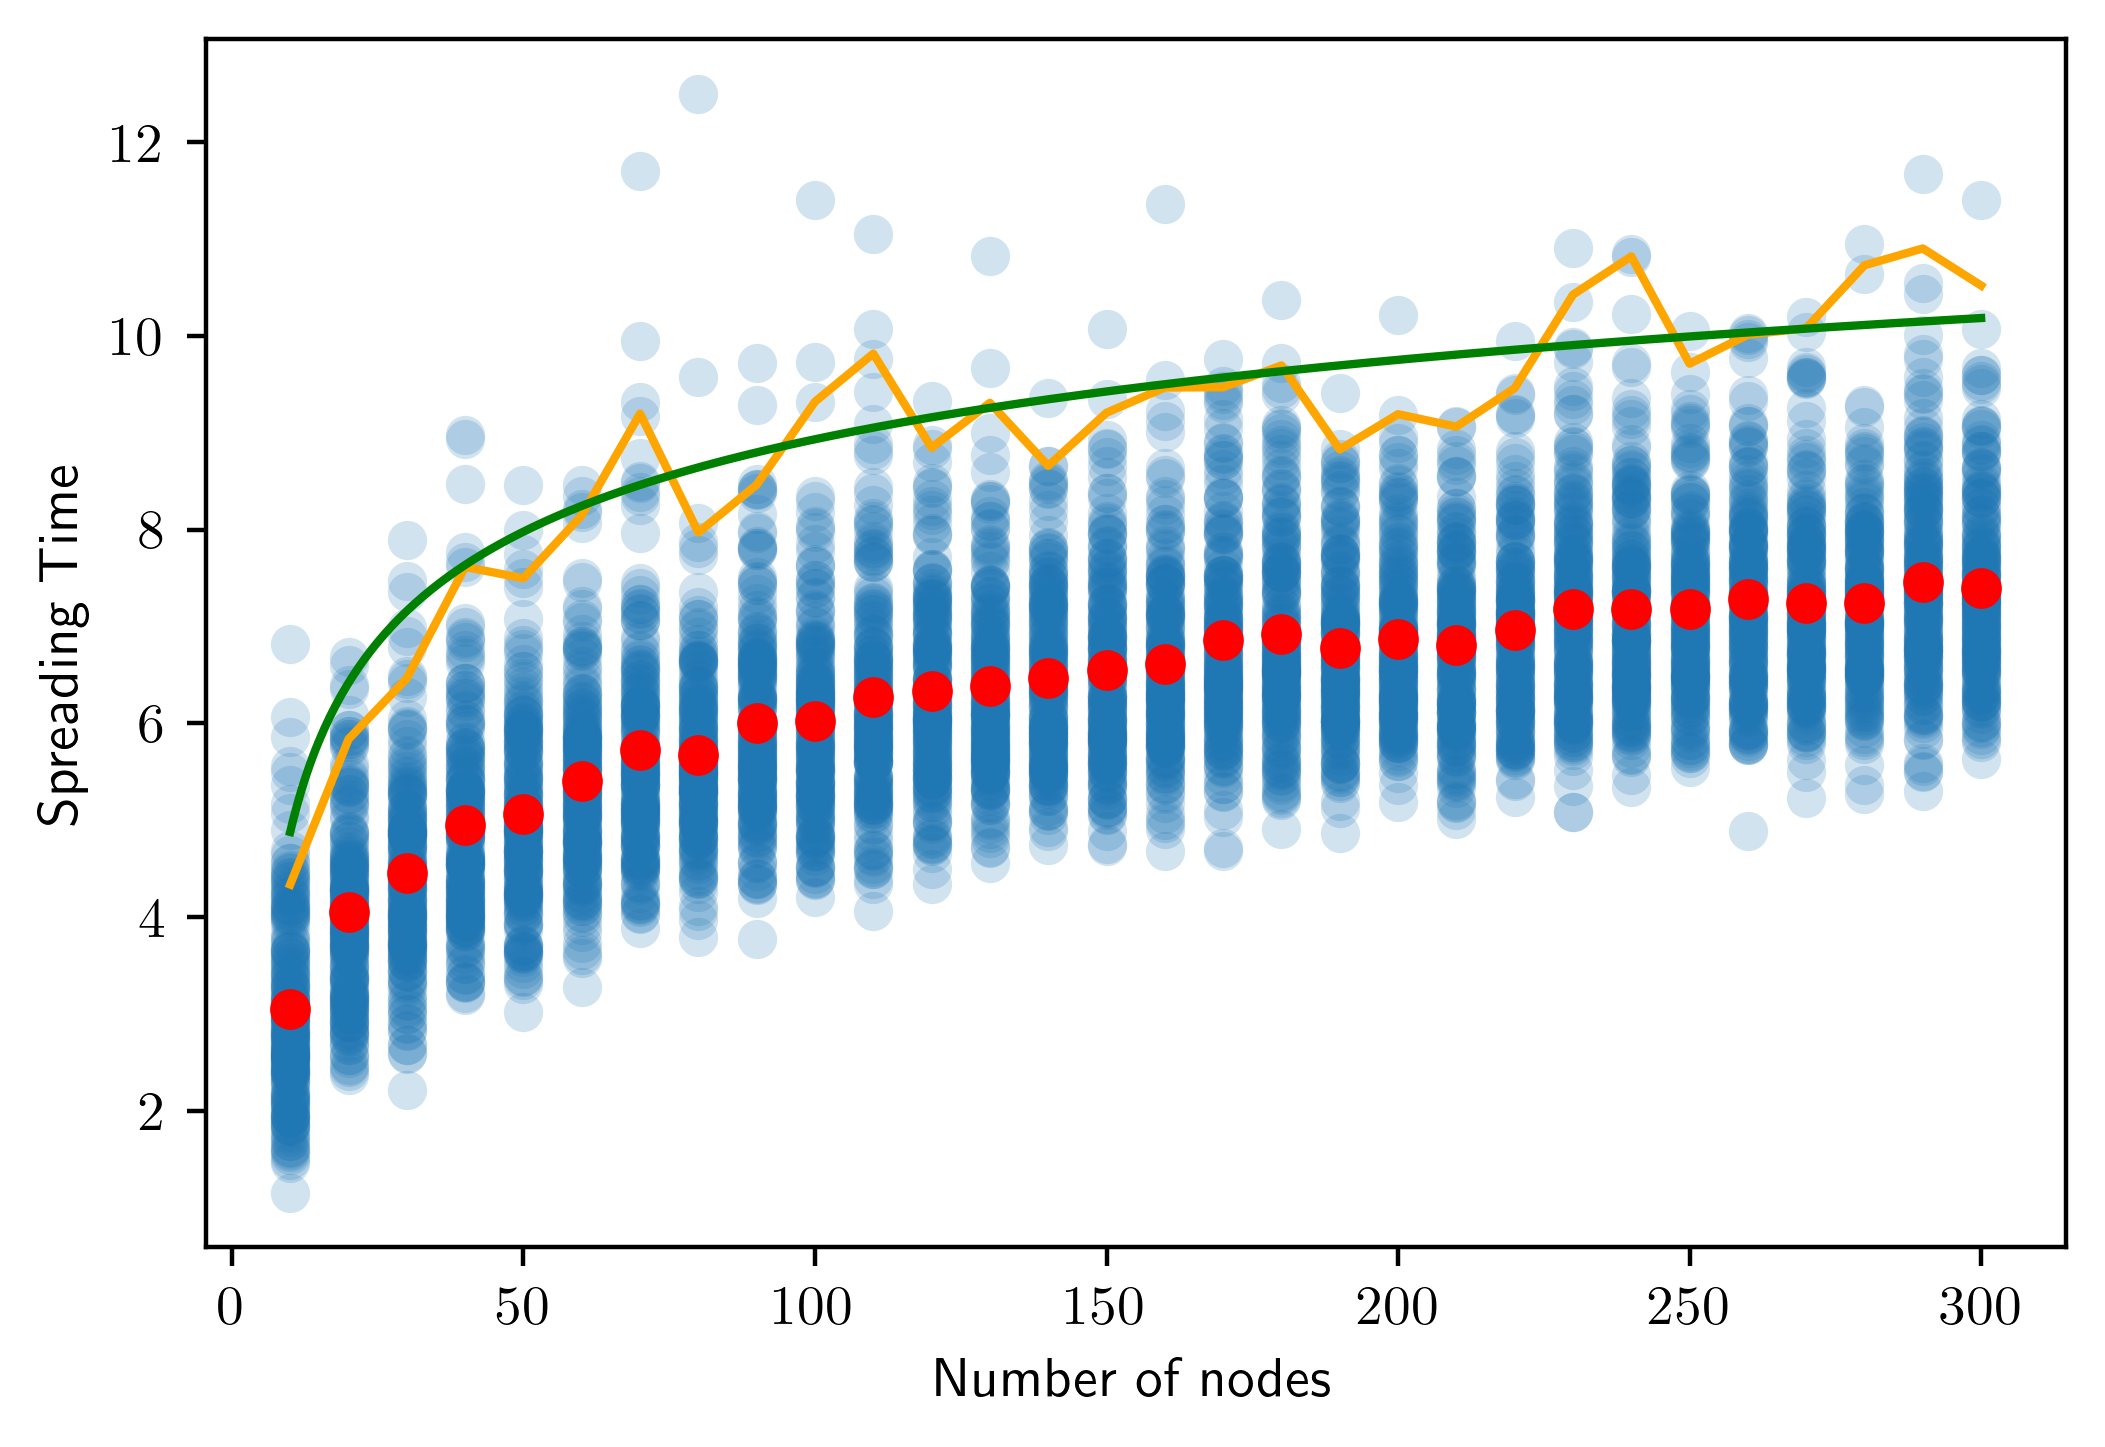
\includegraphics[width=1\textwidth]{./figures/alternating_ring_simulation_results.png}
	\caption{Results of Ring-Complete Alternating Network spreading time simulations}
	\label{fig:alternatingSimResults}
\end{figure}

The scatter plot in Figure \ref{fig:alternatingSimResults} displays the results rumour spreading on $\mathcal{A}$. Each blue point in the plot represents a single simulation, where the $x$ component is the number of nodes in the simulation, and the $y$ component is spreading time. Since the spreading time is random variable, 50 simulations were run for each network size we investigated. The mean of these 50 simulations are plotted in red. % TODO: 50 runs to eliminate varaince of indiviudal runs, bound w.h.p

% TODO: Difference between means and bound -> means fit bound => likely bound works/is tight, expect all points beneath bound don't expect means to follow bound exactly
% TODO: Analysis - what does this sim actually tell us

We now consider an example of a dynamic network where the bound is not tight in scaling. % TODO: Reword

\subsubsection{Shuffled Ring}\label{subsect:shuffledRingAsyncApplication}

We start by introducing the Shuffled Ring Network.

\begin{definition}
	Shuffled Ring Network $\mathcal{S}$

	Let $(G_t)_{t \in \mathbb{N}}$ be the topologies of $\mathcal{S}$. In a shuffled ring network, each $G_t$ is a ring topology (i.e. a single cycle on all the nodes) drawn uniformly at random from the set of all possible ring graphs. 
\end{definition}

\begin{figure}[h]
	\centering
    \begin{subfigure}[b]{0.3\textwidth}
		\centering
		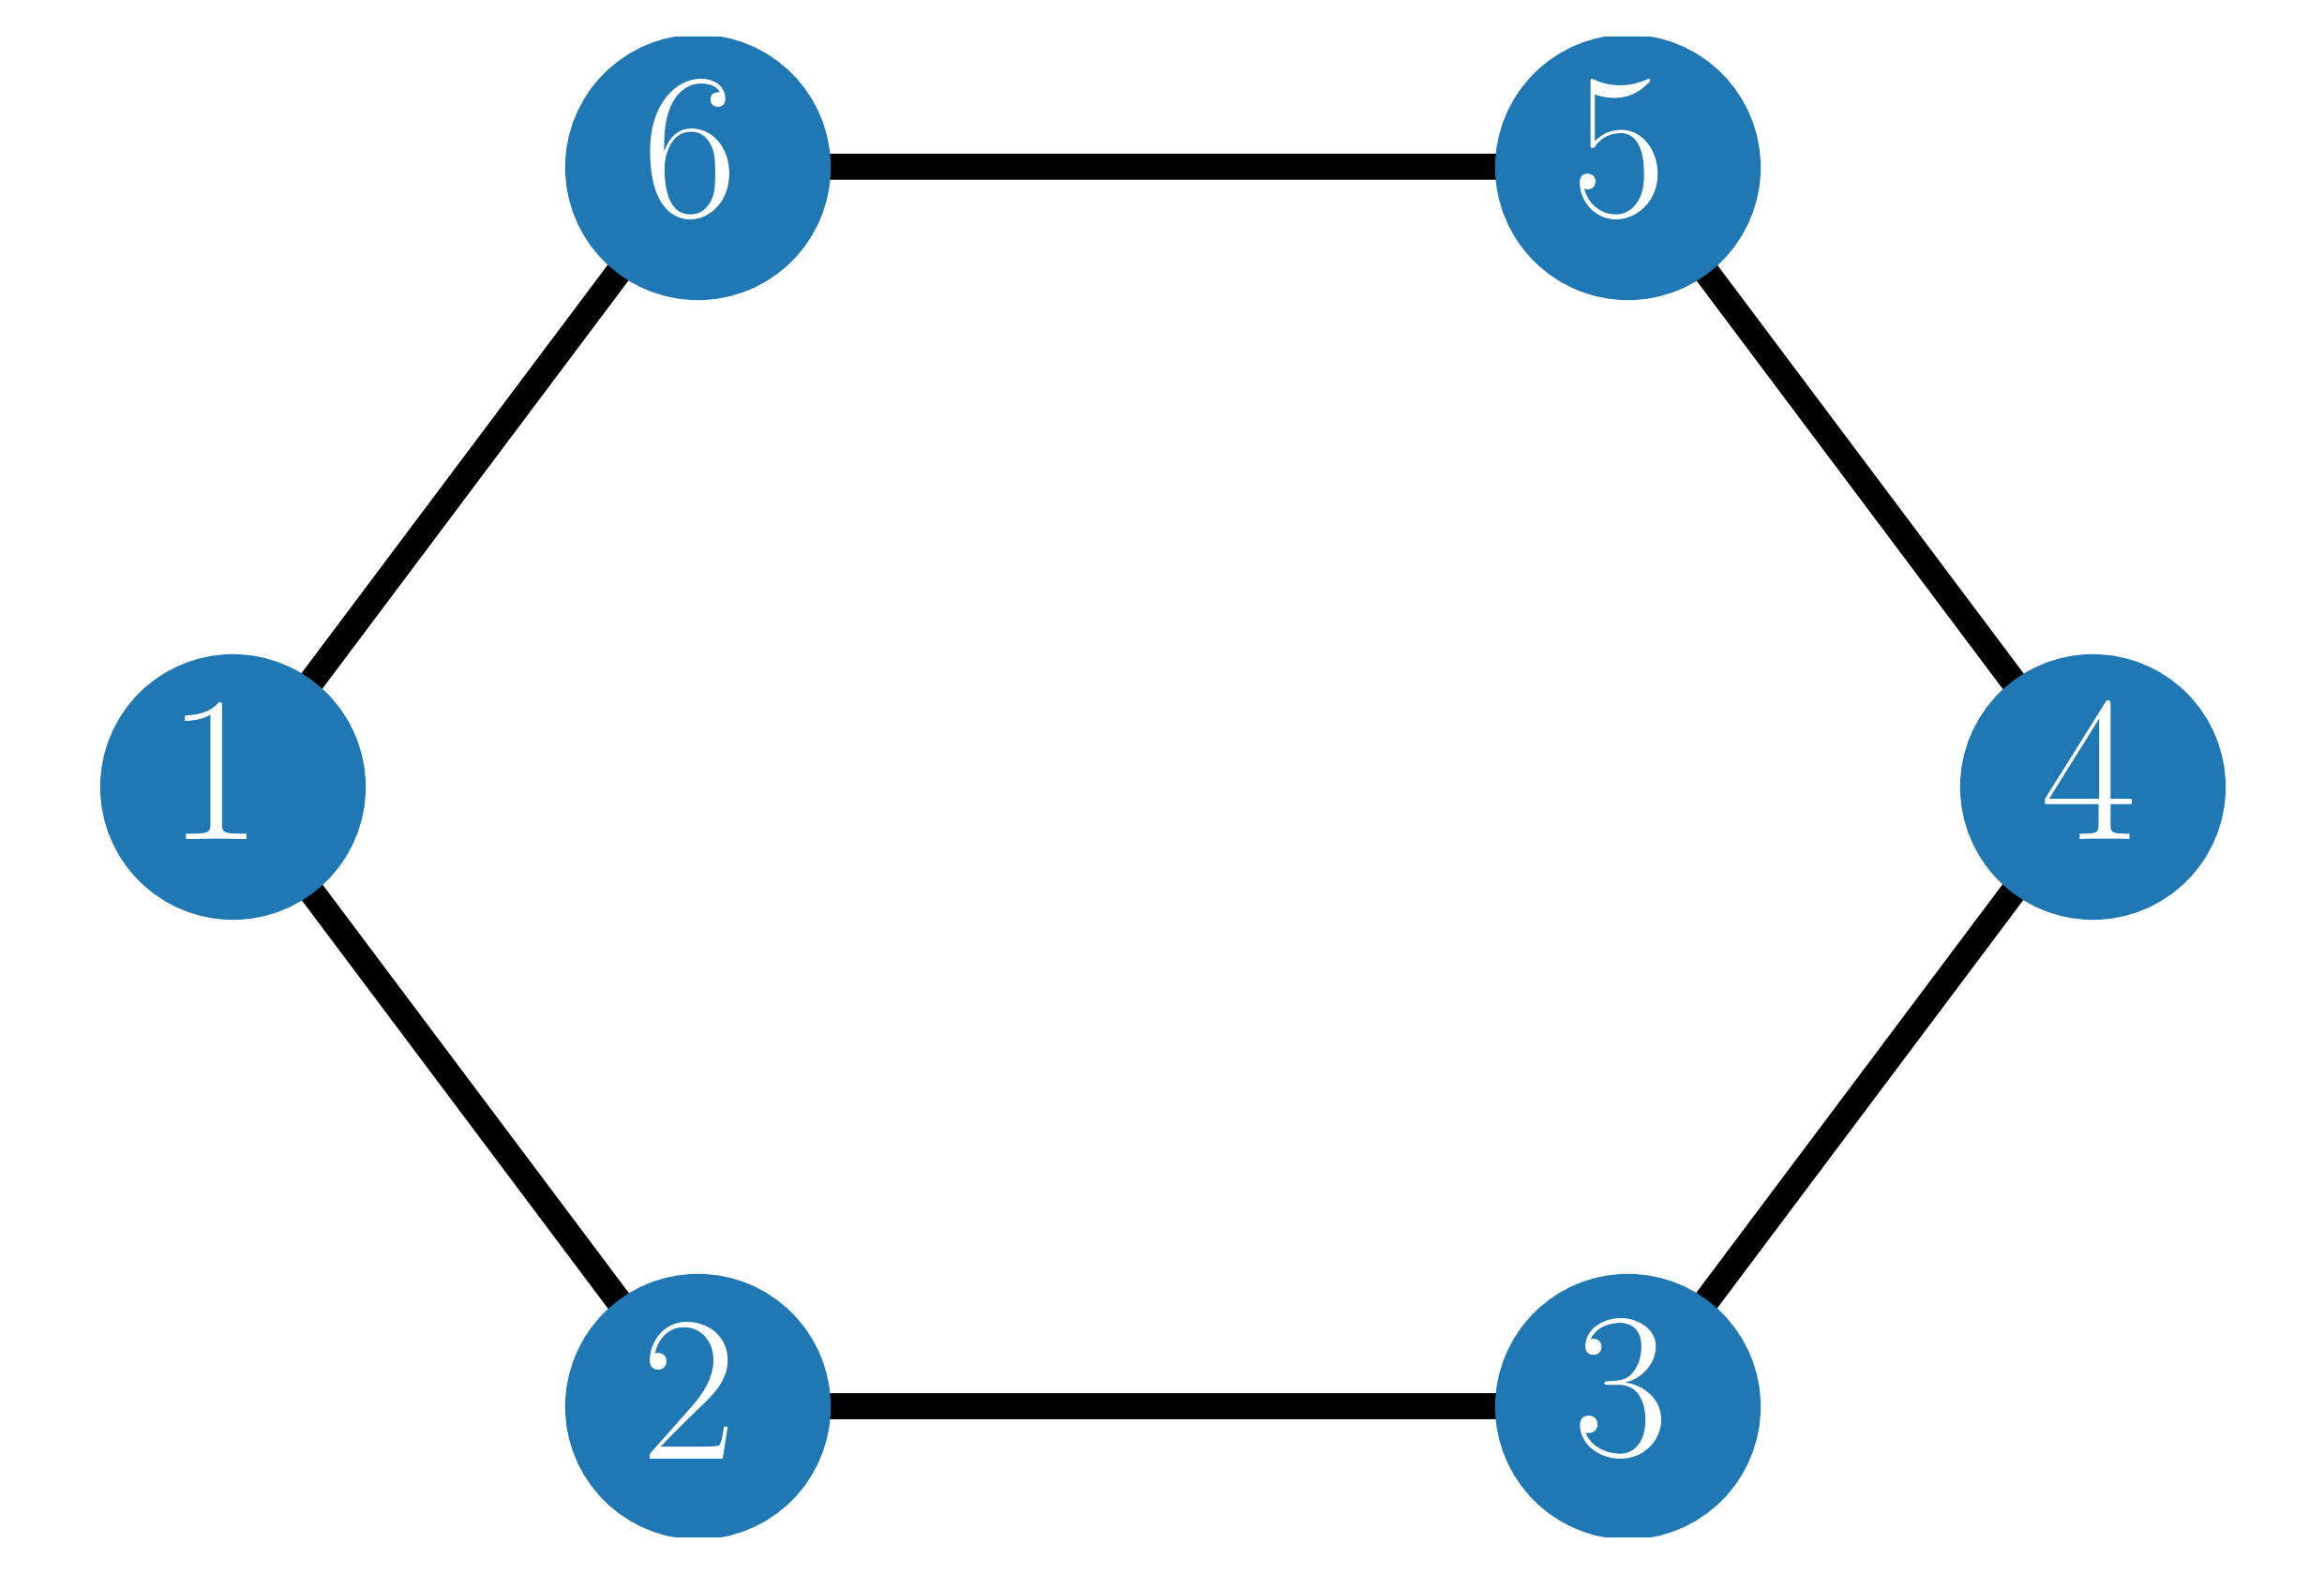
\includegraphics[width=\textwidth]{./figures/shuffled_ring_1.png}
		\caption*{$G_0$}
	\end{subfigure}
	\begin{subfigure}[b]{0.3\textwidth}
		\centering
		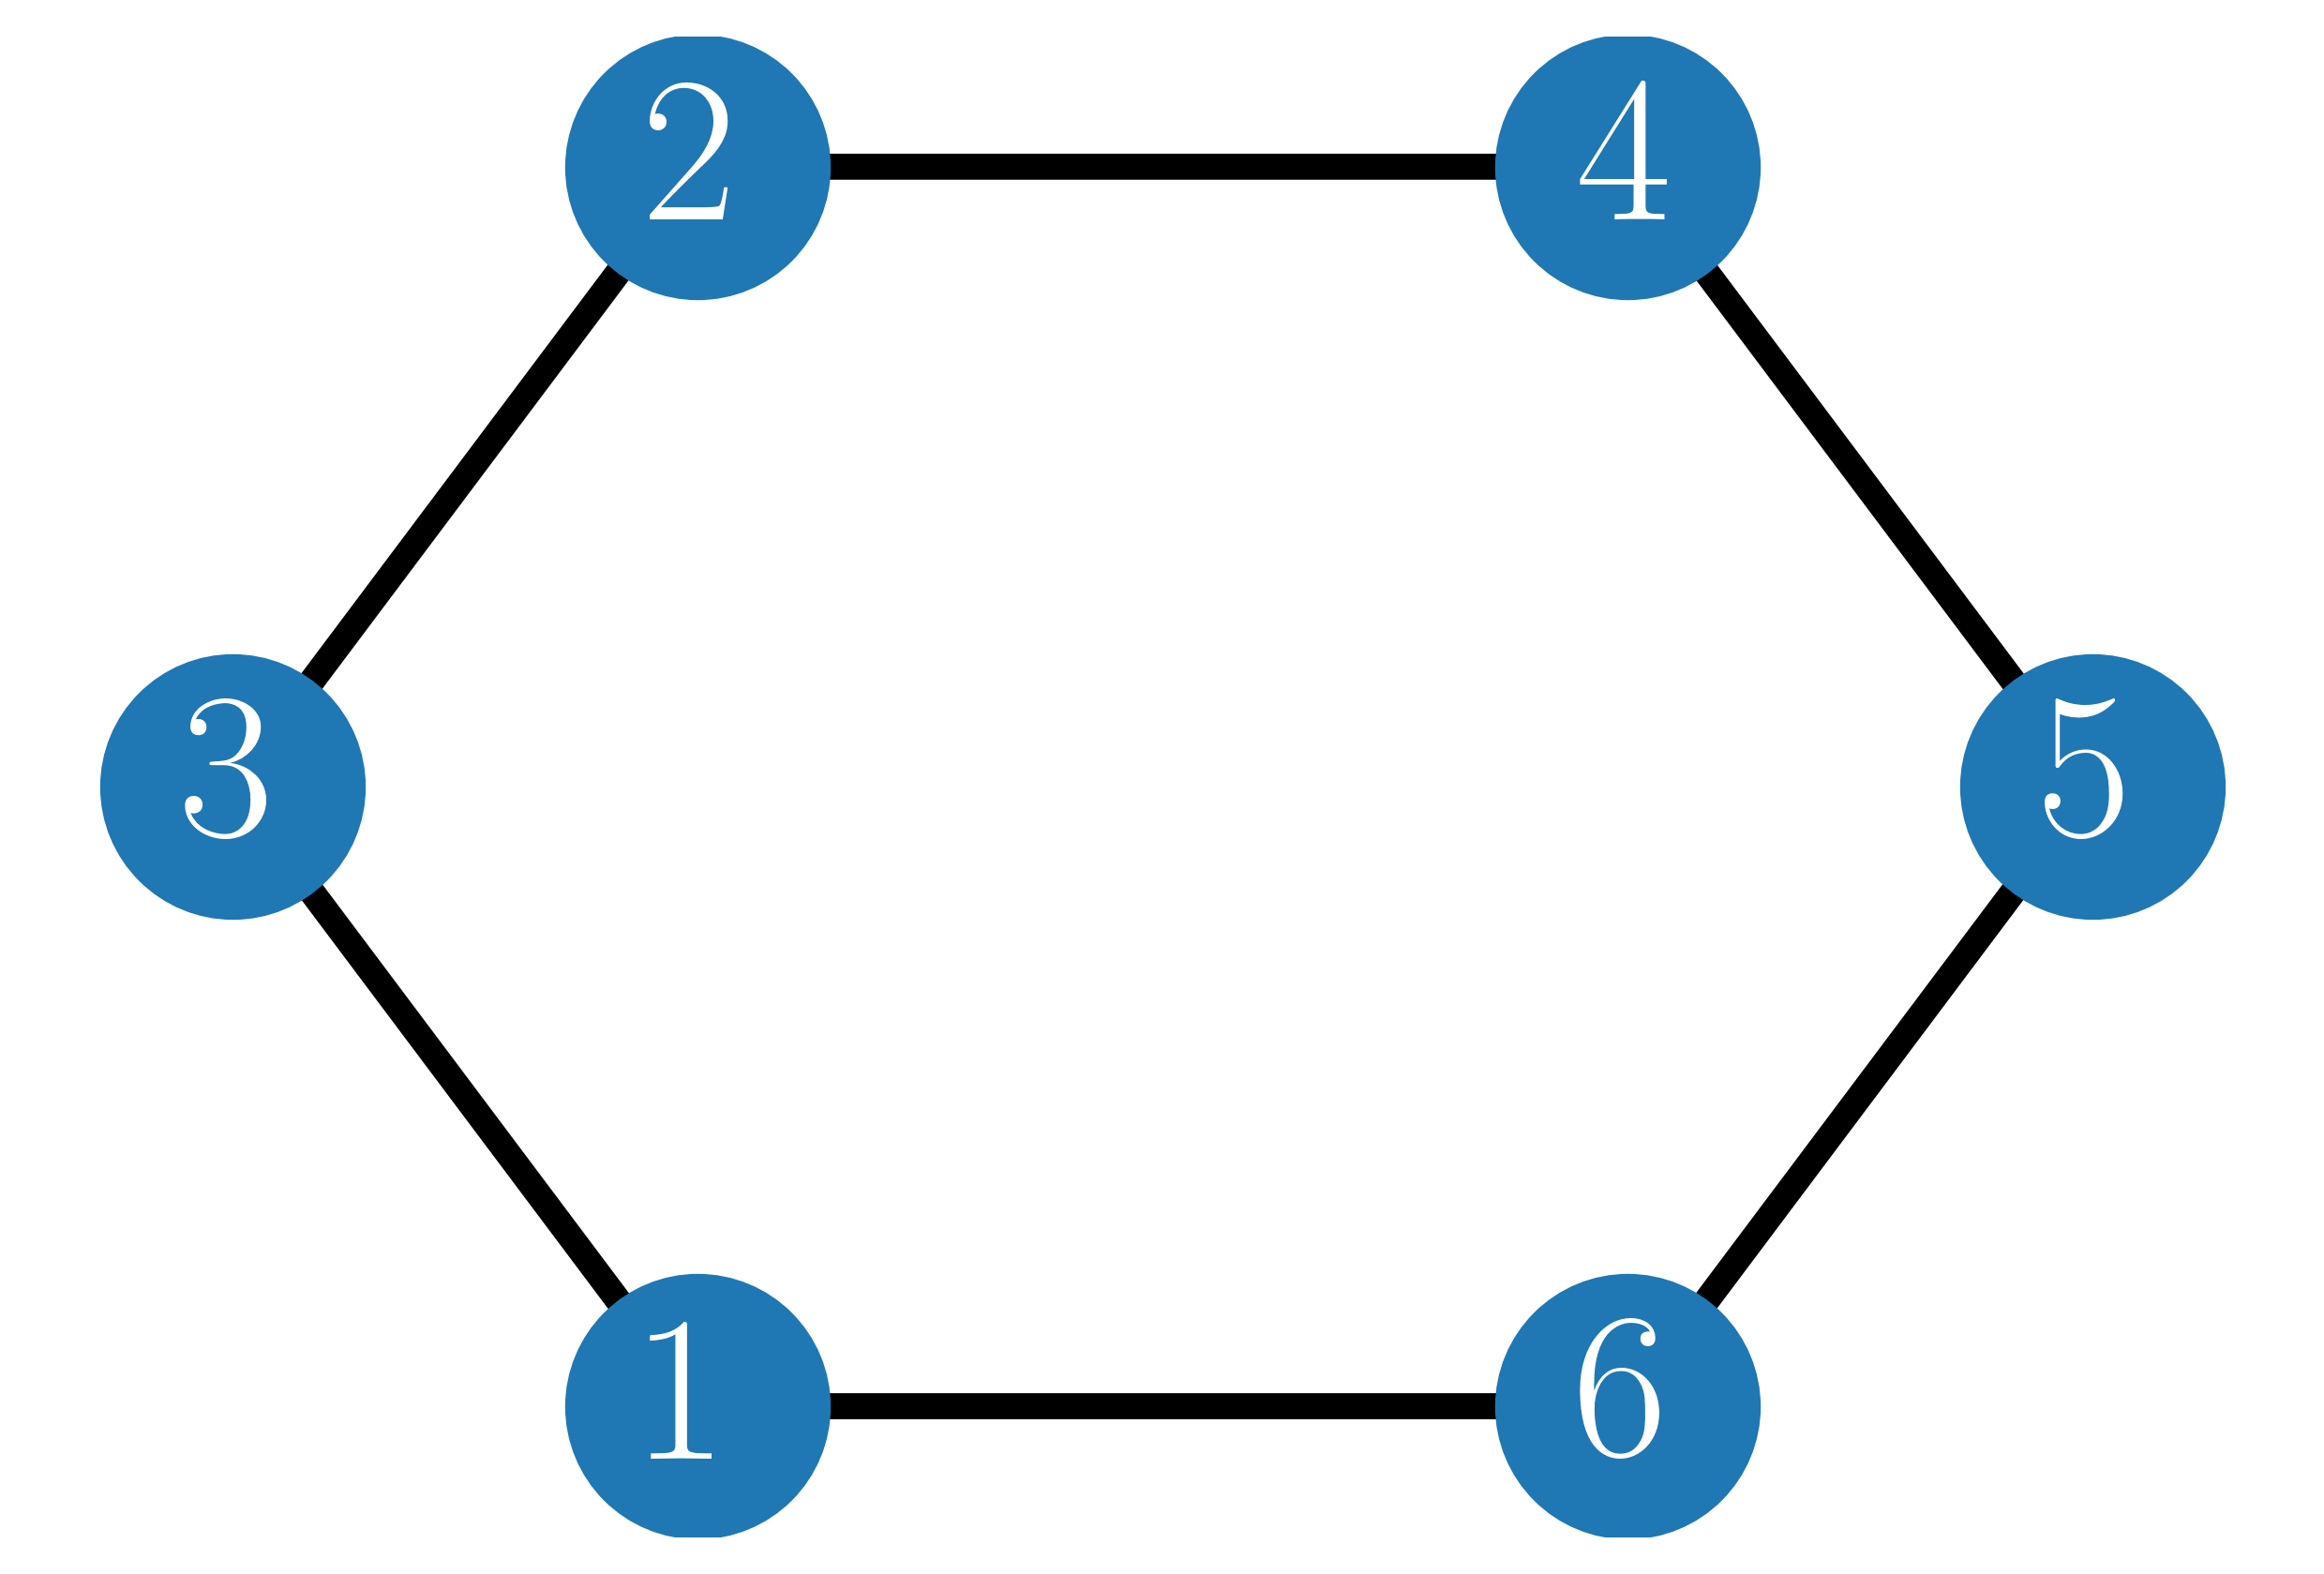
\includegraphics[width=\textwidth]{./figures/shuffled_ring_2.png}
		\caption*{$G_1$}
	\end{subfigure}
	\begin{subfigure}[b]{0.3\textwidth}
		\centering
		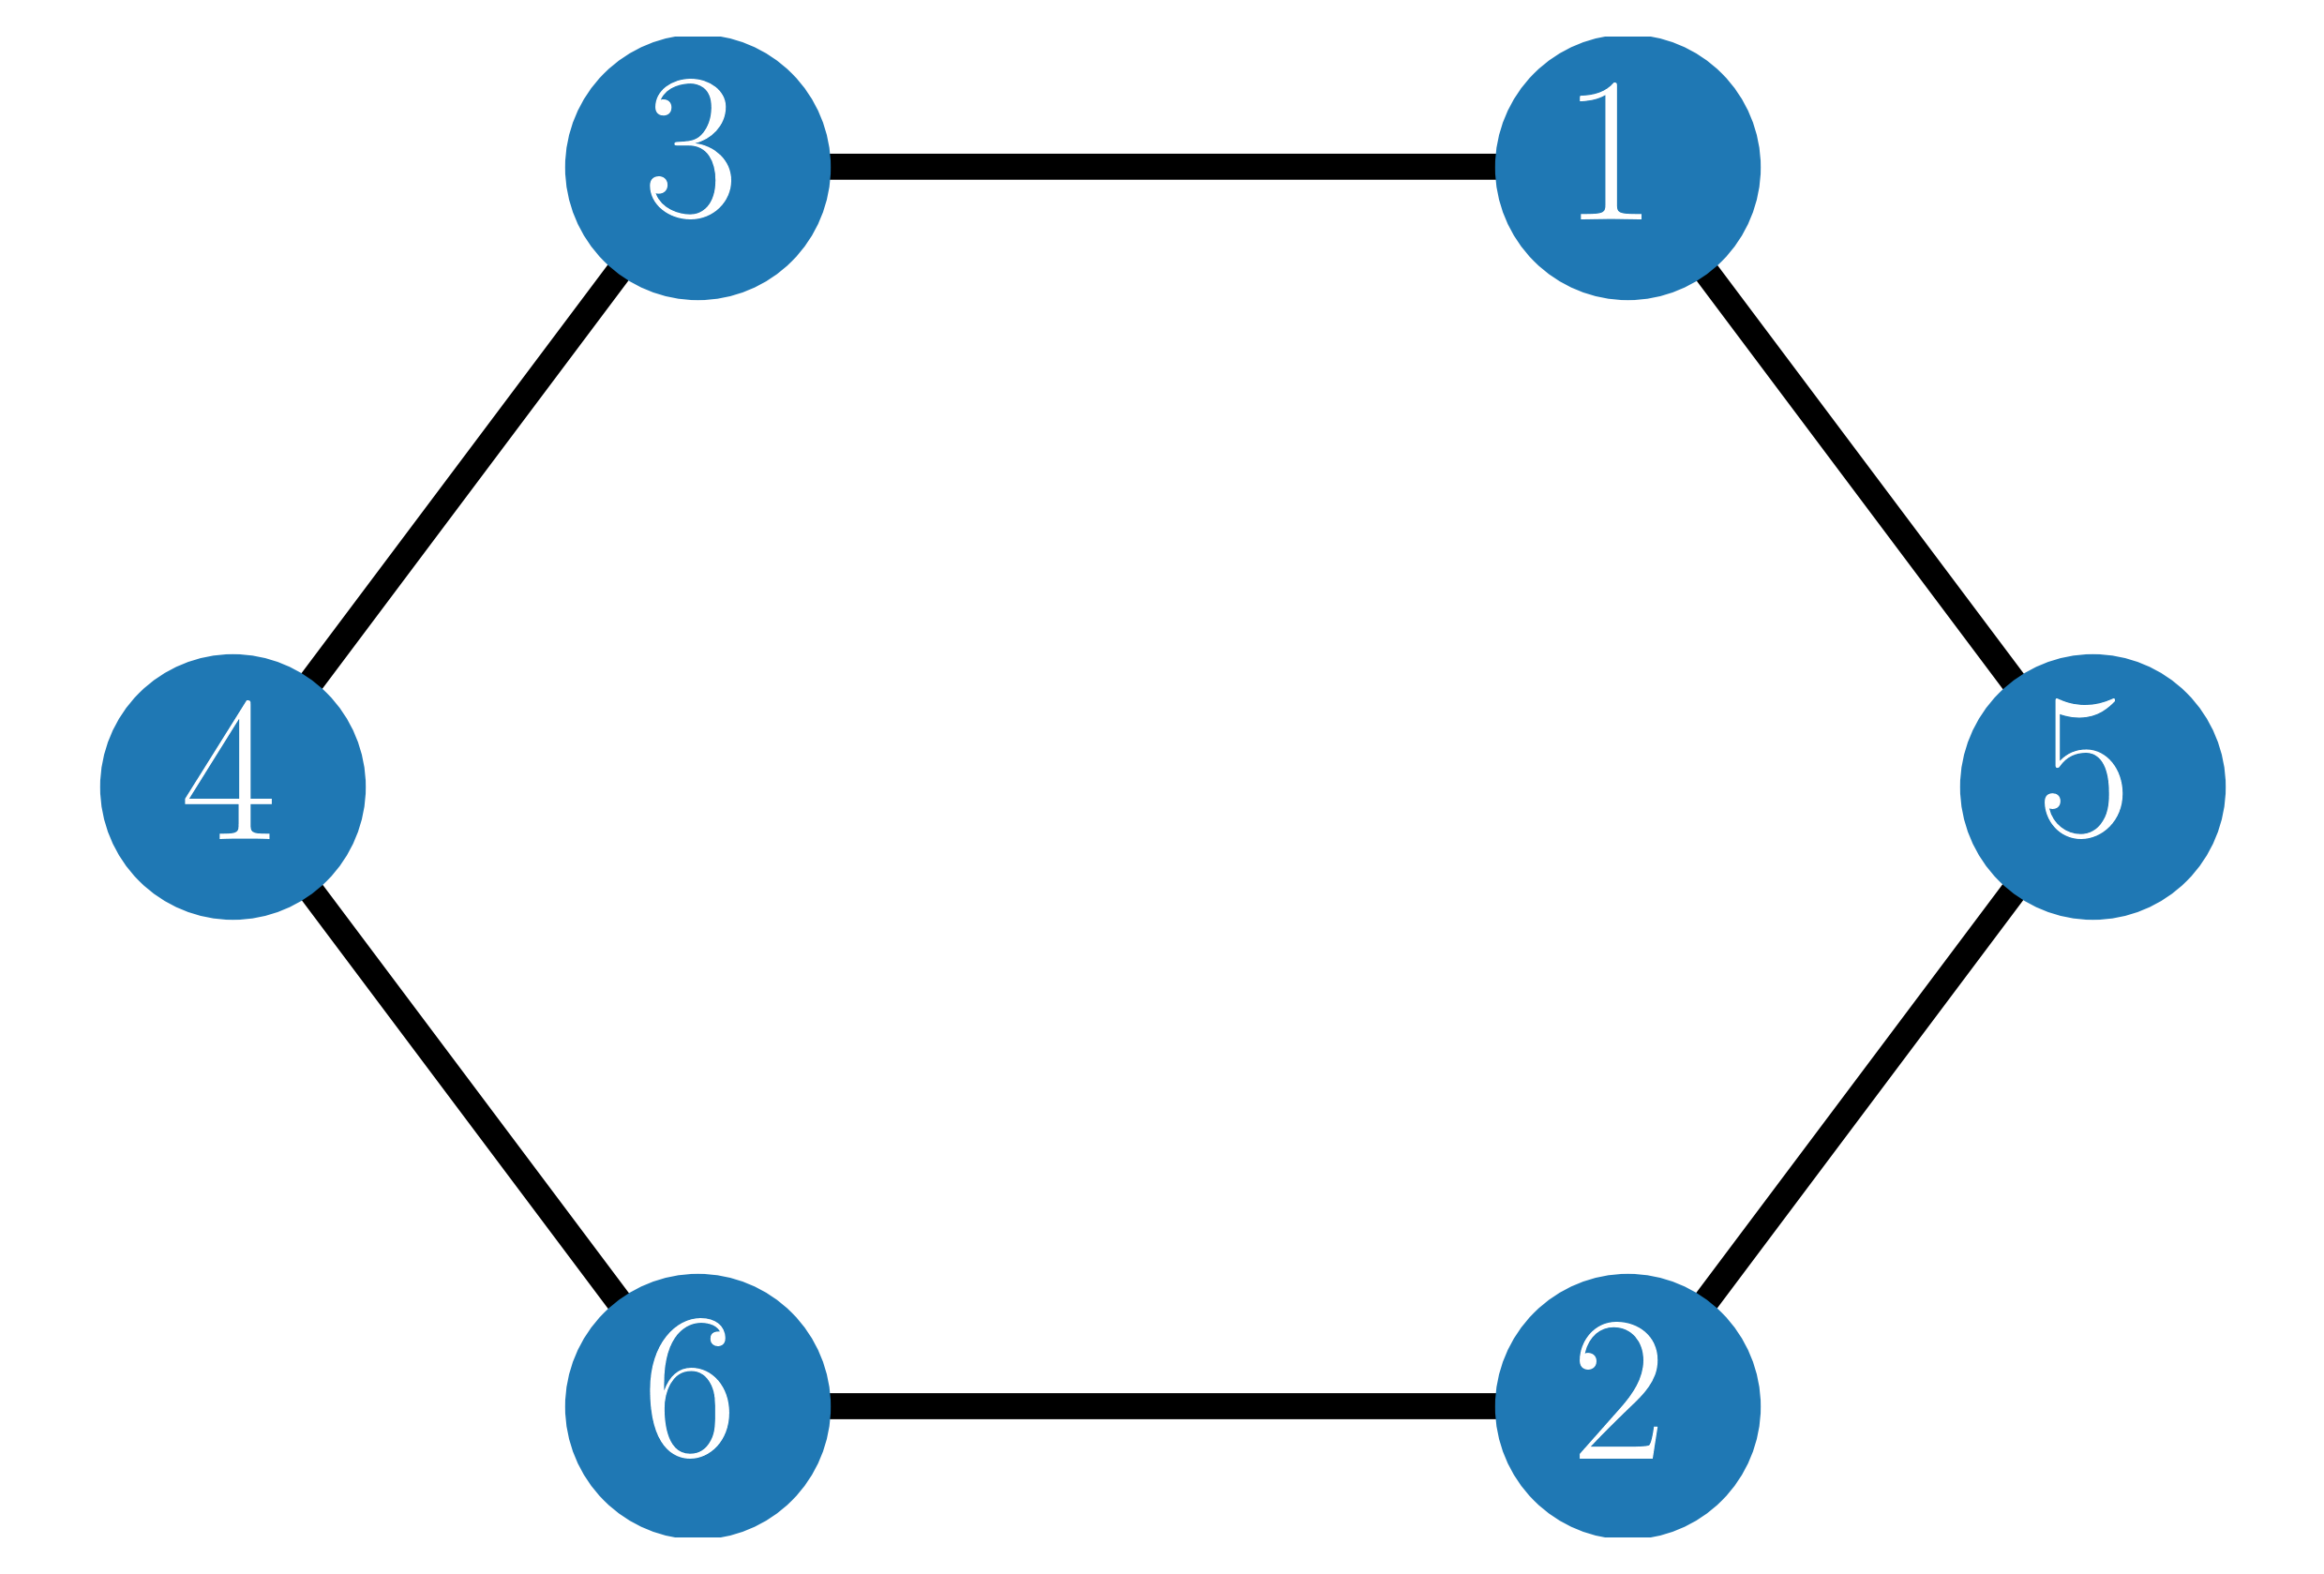
\includegraphics[width=\textwidth]{./figures/shuffled_ring_3.png}
		\caption*{$G_2$}
	\end{subfigure}
	\caption{First three topologies of an example Shuffled Ring Network}
	\label{fig:shuffledRingExample}
\end{figure}

In Figure \ref{fig:shuffledRingExample} we see an example of the first three topologies in a shuffled ring network. Each topology is always a ring, but the order of the nodes is selected uniformly at random each round.

We now use Theorem \ref{theorem:AsyncUpperBound} to bound the spreading time on the Shuffled Ring Network.

\begin{theorem}
	w.h.p the spreading time of Algorithm \ref{NodeCentricAsyncAlgorithm} on the Shuffled Ring Network is at most $\mathcal{O}(n \log n)$.
\end{theorem}

\begin{proof}
	By Theorem \ref{theorem:AsyncUpperBound} we have that w.h.p the rumour spreads in time at most 
	$$
		\min \left\{t : \sum_{k=0}^t \Phi(G_k)\rho(G_k) \geq C \log n \right\} 
	$$
	By computing this quantity explicitly with the conductance and diligence results for the ring graph from Theorem \ref{theorem:ringCompleteAsyncBound} we obtain
	\begin{align*}
		\min \left\{t : \sum_{k=0}^t \Phi(G_k)\rho(G_k) \geq C \log n \right\} 
		&= \min \left\{t : t \Phi(R)\rho(R) \geq C \log n \right\} \\
		&= \min \left\{t : t \Phi(R)\rho(R) \geq C \log n \right\} \\
		&= \ceil{\frac{C \log n}{\Phi(R)\rho(R)}} \\
		&= \ceil{\frac{C}{2}n \log n}
	\end{align*}
\end{proof}

We see that the bound we obtain for the spreading time on the Shuffled Ring Network is a factor of $n$ larger than the Ring-Complete Alternating Network, due to the loss of the high-connectivity complete topologies. % TODO: More exposition/analysis here?

Now we compare the bound we have obtained with simulated spreading times on the Shuffled Ring Network.

\begin{figure}[h]
	\centering
	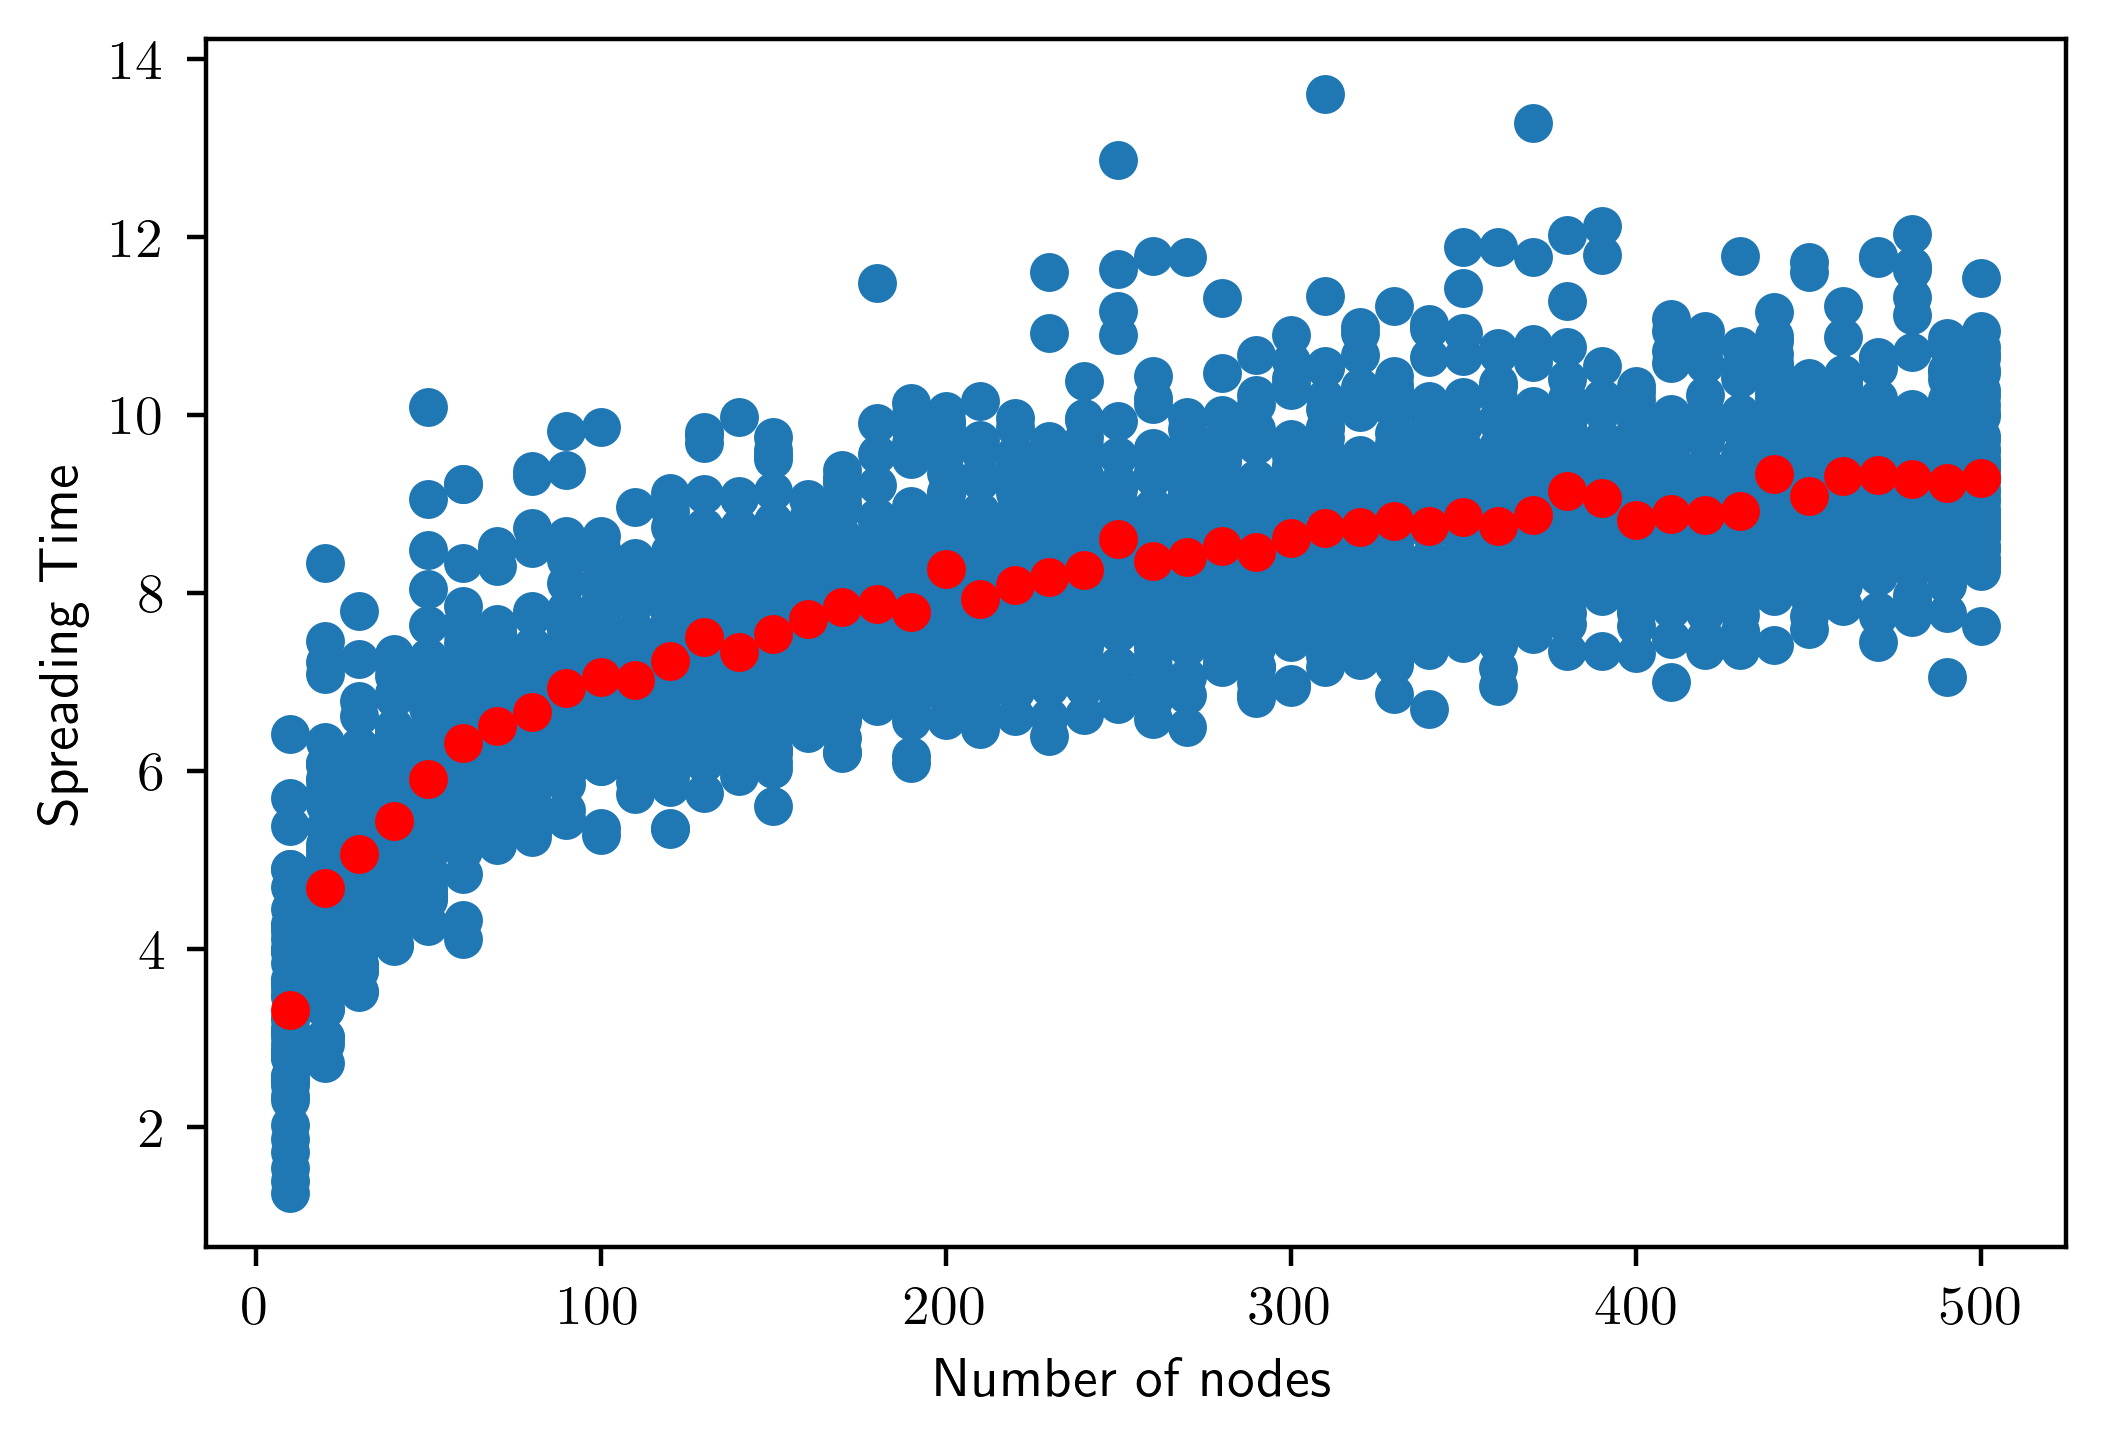
\includegraphics[width=1\textwidth]{./figures/shuffle_ring_simulation_results.png}
	\caption{Results of shuffled ring spreading time simulations}
	\label{fig:shuffleRingSimResults}
\end{figure}

We see from Figure \ref{fig:shuffledRingExample} that the spreading times of the Shuffled Ring Network grow logarithmically in the size of the network. % TODO: Justify rigourouly, generate "closeness" metric to true log n?
Thus, the $\mathcal{O}(n \log n)$ bound given by Theorem $\ref{theorem:AsyncUpperBound}$ is larger by a factor of $n$ in scaling. 
% TODO: Justify more - bound is weak, doesn't give much information, less useful, motivates investigation into why the bound is weak in this case, and are there other cases where it is also weak?, can we tighten it?
But why is it the case that the bound is weak for the Shuffled Ring Network? 

To answer this question, we investigate the spreading time on the static ring graph.

\subsubsection{Static Ring}

\begin{definition}
	Static Ring Network $\mathcal{R}$

	\noindent
	Let $R$ be a cycle graph on $n$ nodes. The Static Ring Network is the network consisting of the same ring $R$ for every topology, i.e. $\mathcal{R} = (G_t)_{t \in \mathbb{N}}$ where $G_t = R$ for all $t \in \mathbb{N}$. 
\end{definition}

\begin{theorem}\label{theorem:staticRingAsyncBound}
	w.h.p the spreading time of Algorithm \ref{NodeCentricAsyncAlgorithm} on the Static Ring Network is at most $\mathcal{O}(n \log n)$.
\end{theorem}

\begin{proof}
	We notice that in each round the topologies of Shuffled Ring Network and Static Ring Network networks are identical up to the renaming of nodes. Since these two networks have the same structure (namely a ring graph for all topologies), they also have the same conductance and diligence in each round. Hence, Theorem \ref{theorem:AsyncUpperBound} yields the same bound for the Static Ring Network as the Shuffled Ring Network. % TODO: More details
\end{proof}

% TODO: OUR bound holds for all networks with the same topologies up to renaming of nodes. 

Now we investigate the simulated spreading times on the Static Ring Graph.

\begin{figure}[h]
	\centering
	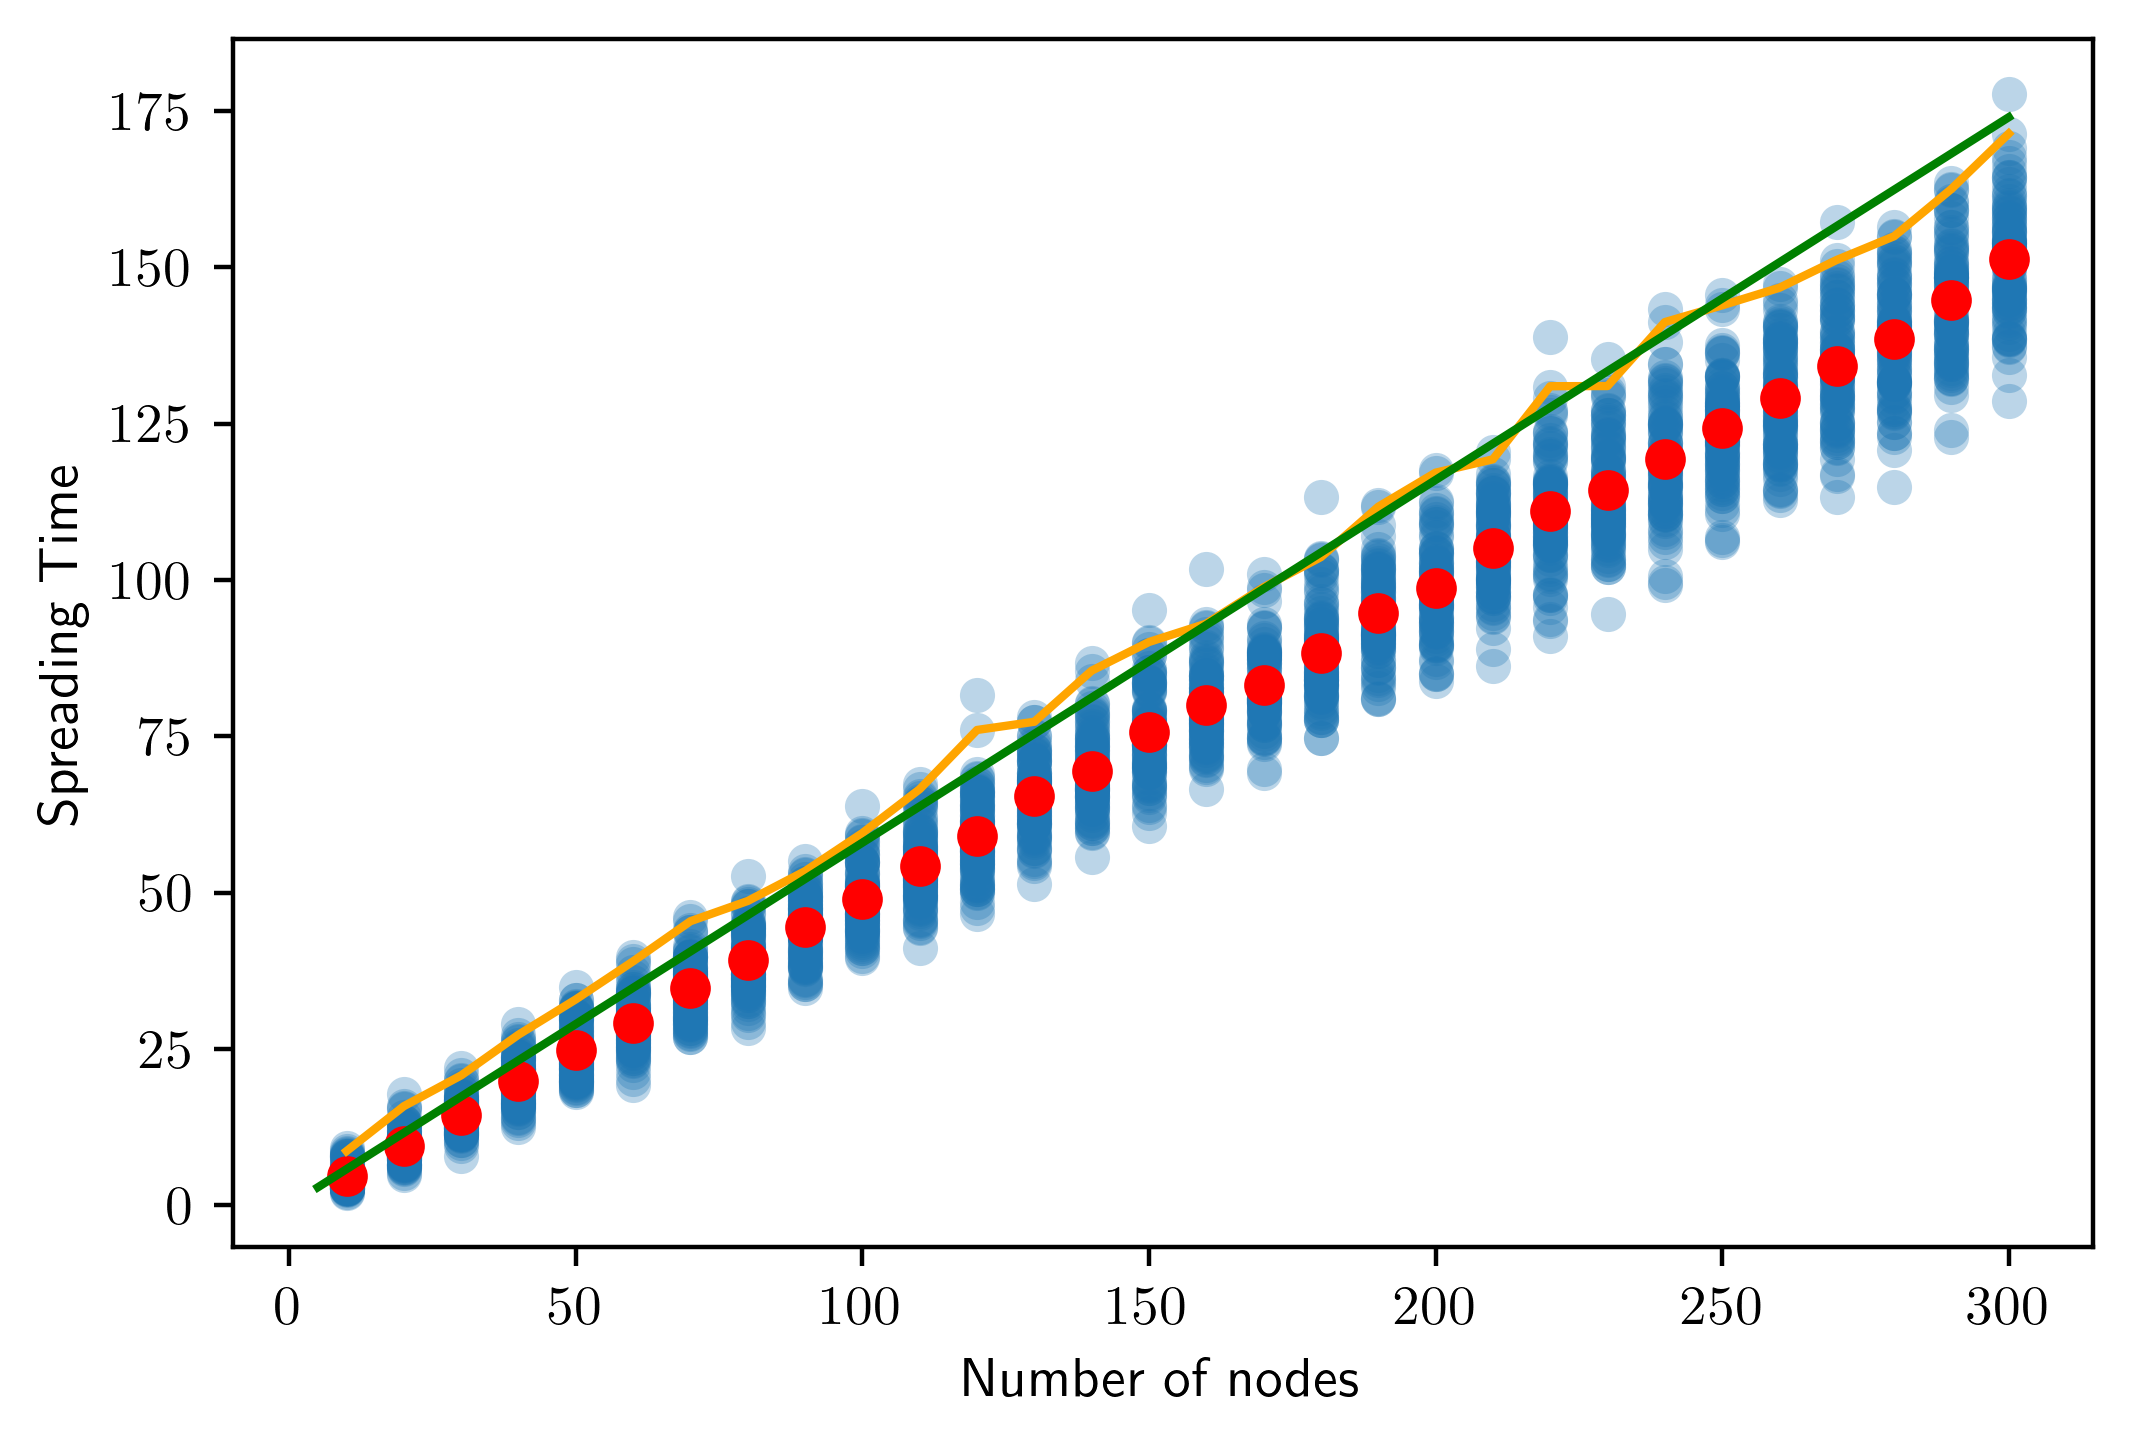
\includegraphics[width=1\textwidth]{./figures/static_ring_simulation_results.png}
	\caption{Results of static ring spreading time simulations}
	\label{fig:staticRingSimResults}
\end{figure}

We see from the simulations on the Static Ring Graph that the spreading time grows linearly with the number of nodes in the network. Notice that this is significantly slower than the logarithmic growth seen in the Shuffled Ring simulations, despite both networks having isomorphic topologies. %TODO: Define ismorhpic for graphs and then networks

In this case, the $\mathcal{O}(n \log n)$ bound given by Theorem \ref{theorem:AsyncUpperBound} is much tighter, and is only a factor of $\mathcal{O}(\log n)$ larger than the simulated spreading times.
% TODO: Finish above when established link between bound holding w.h.p and being in line with simulations.

We investigate why the rumour spreads faster on the Shuffled Ring Network by comparing how the rumour spreads in the Shuffled Ring and Static Ring networks. % TODO: Redundant sentance?

% TODO: Talk about the general behaviour when dicussing how made simulations earlier? Bit of a jump here
By Theorem [TODO:CITE EXPONENTIAL CLOCK THEOREM], we can interpret the operation of Algorithm \ref{NodeCentricAsyncAlgorithm} as picking a node at random when an exponential clock of rate $n$ ticks, % TODO: Change ticks?
then picking a random neighbour to exchange the rumour with. If one of the nodes is aware of the rumour and the other is not, the uninformed node is made aware of the rumour, which we call a "spreading event". We denote the edges along which the rumour can spread (i.e. the edges connecting informed and uninformed nodes) as "active", and the remaining edges as "inactive".
% TODO: INCLUDE THIS? Recall that the rumour only spreads if the chosen edge connects an informed node to an uninformed node. 
In the ring topology all nodes have the same degree, so we can further simplify the interpretation of the spreading process as choosing an edge uniformly at random when an exponential clock of rate $n$ ticks. Thus, the greater the proportion of active edges to inactive edges, the greater the probability that the chosen edge is active, and triggers a spreading event. More frequent spreading events in turn yield lower spreading times. 


\begin{figure}[h]
	\centering
	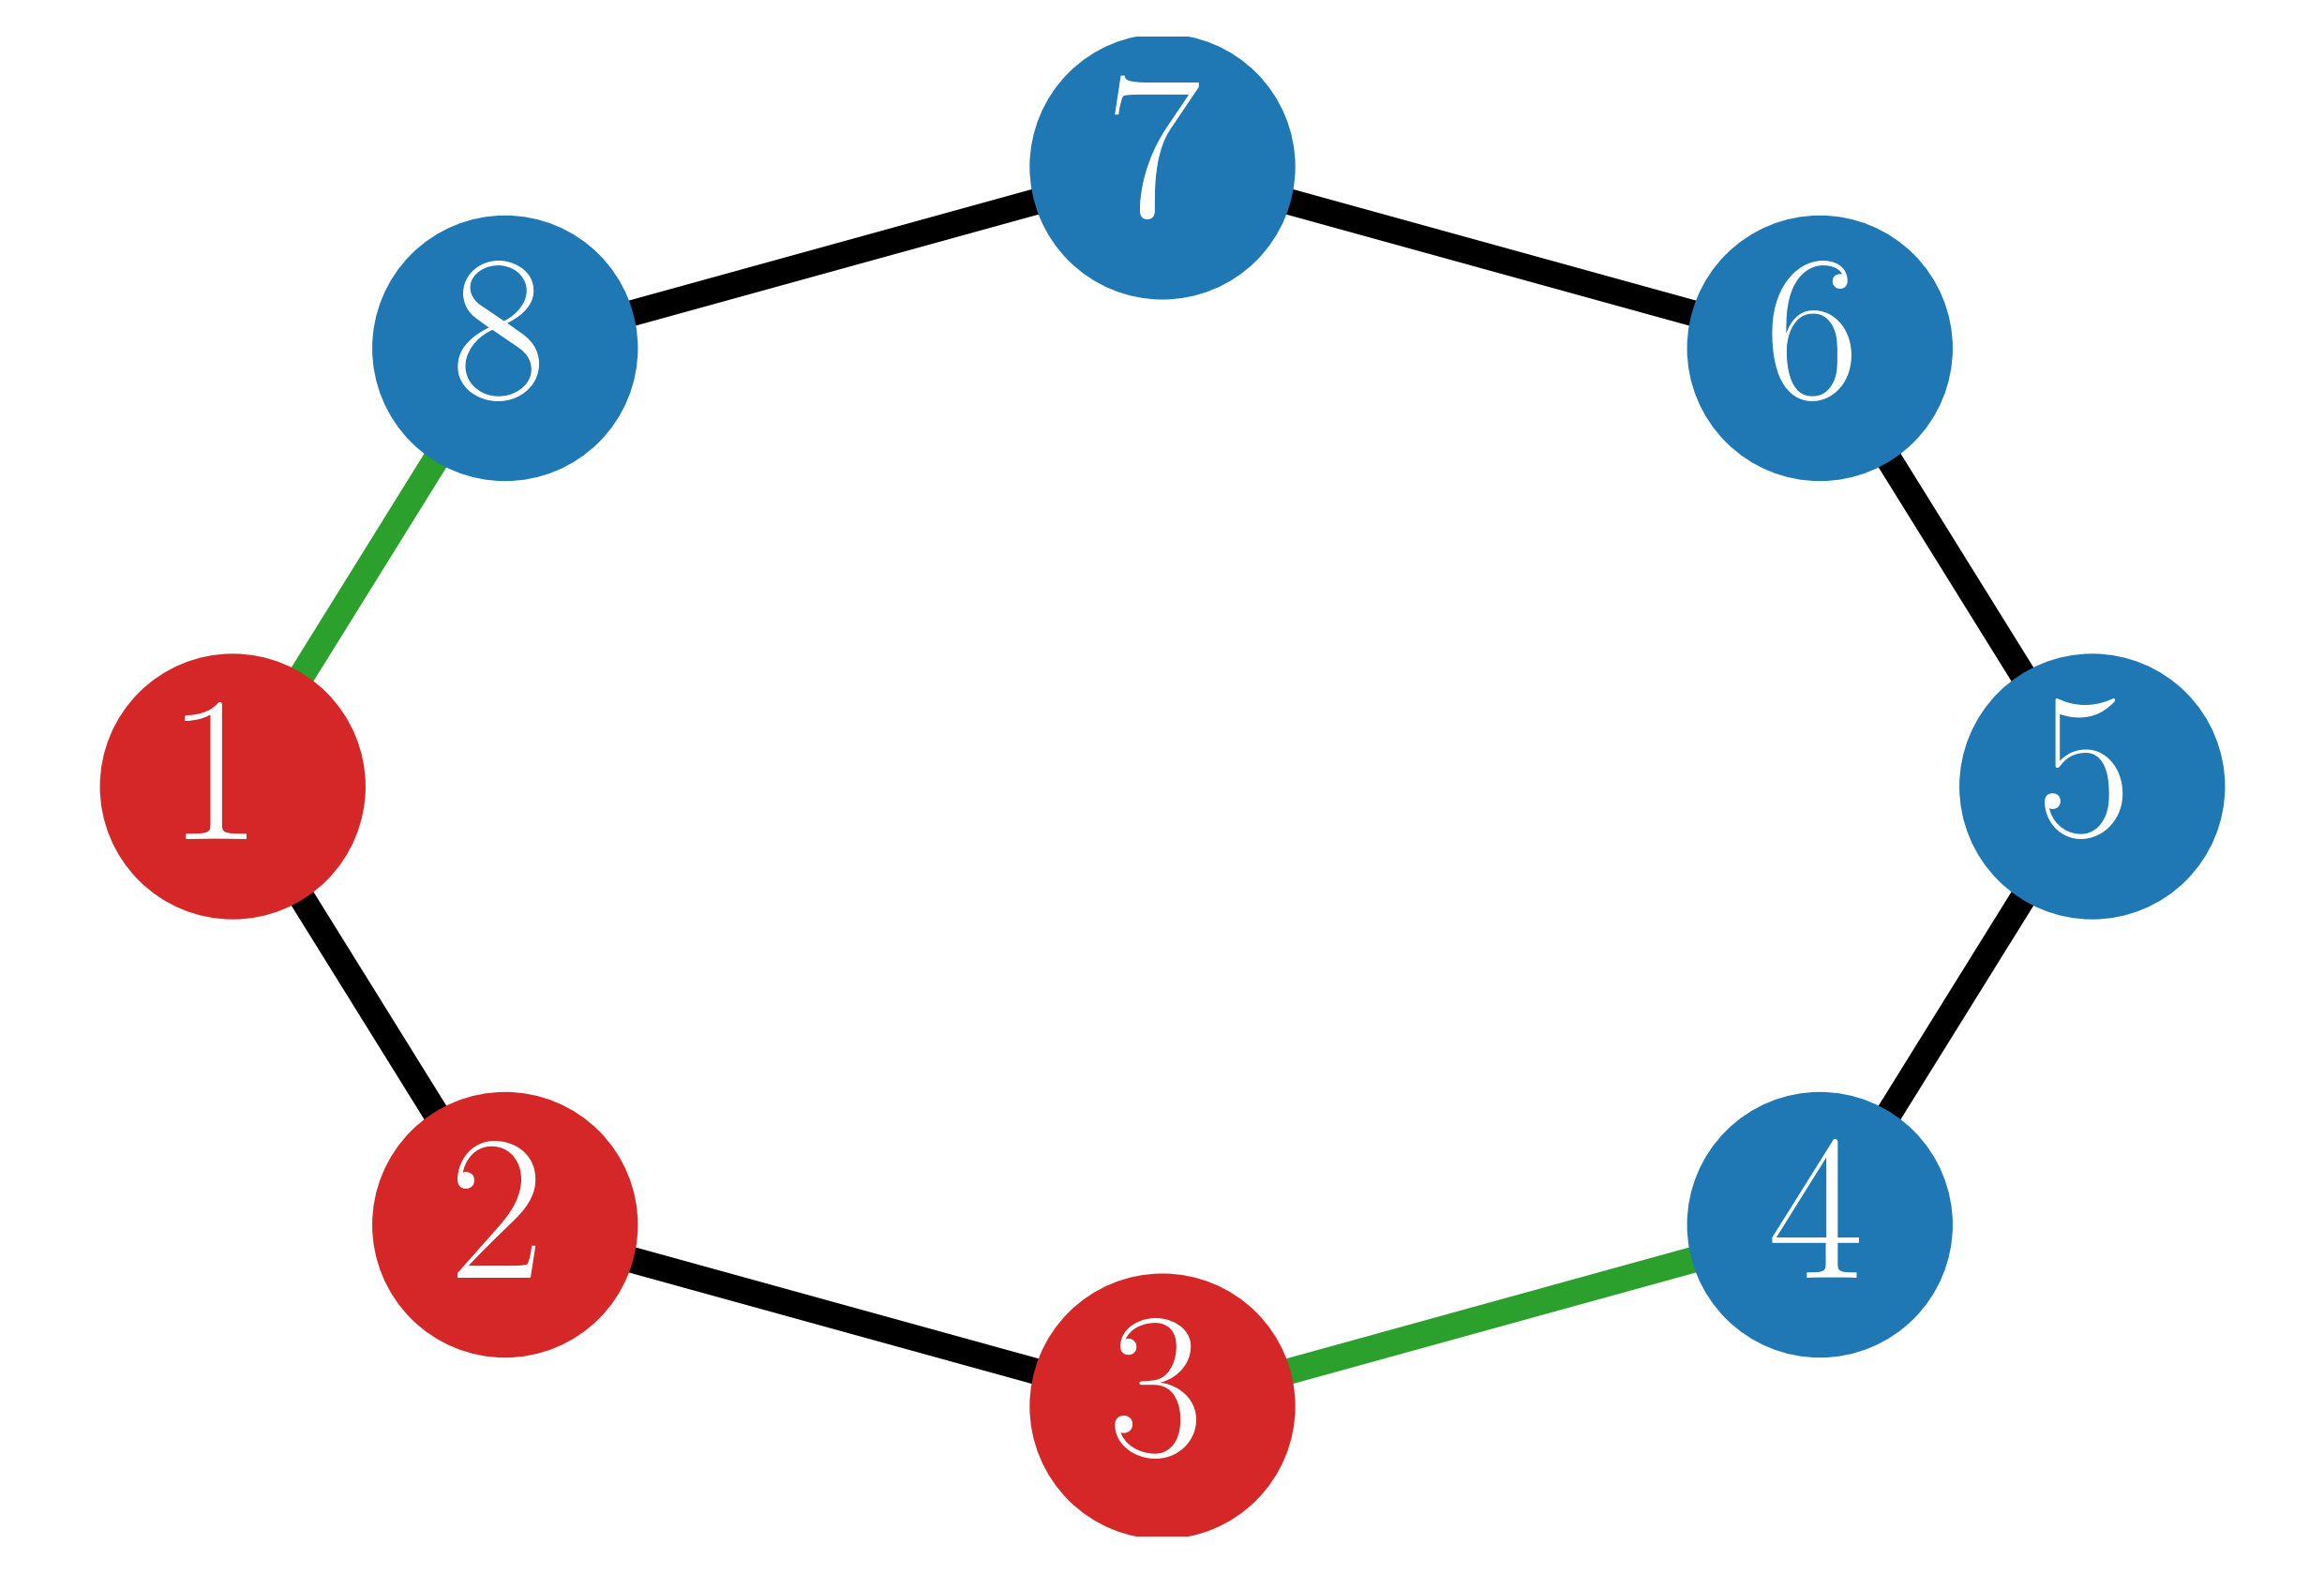
\includegraphics[width=0.49\textwidth]{./figures/static_ring_example_spread.png}
	\caption{Example rumour spread on the Static Ring Network}
	\label{fig:staticRingExampleSpread}
\end{figure}

% TODO: Introduce active edges in static network section

In the Static Ring Network, we find that at all times there are only two active edges, namely the two edges connecting the contiguous set of informed nodes to the uninformed nodes.  This is illustrated in Figure \ref{fig:staticRingExampleSpread}, where red nodes are aware of the rumour, blue nodes are not aware of the rumour, and green edges highlight active connections along which the rumour could spread.

% TODO: Each edge chosen uniformly at random as all same degree. static graph always 2 "active" edges. huffled grpah number of active edges can increase

\begin{figure}[h]
	\centering
    \begin{subfigure}[b]{0.49\textwidth}
		\centering
		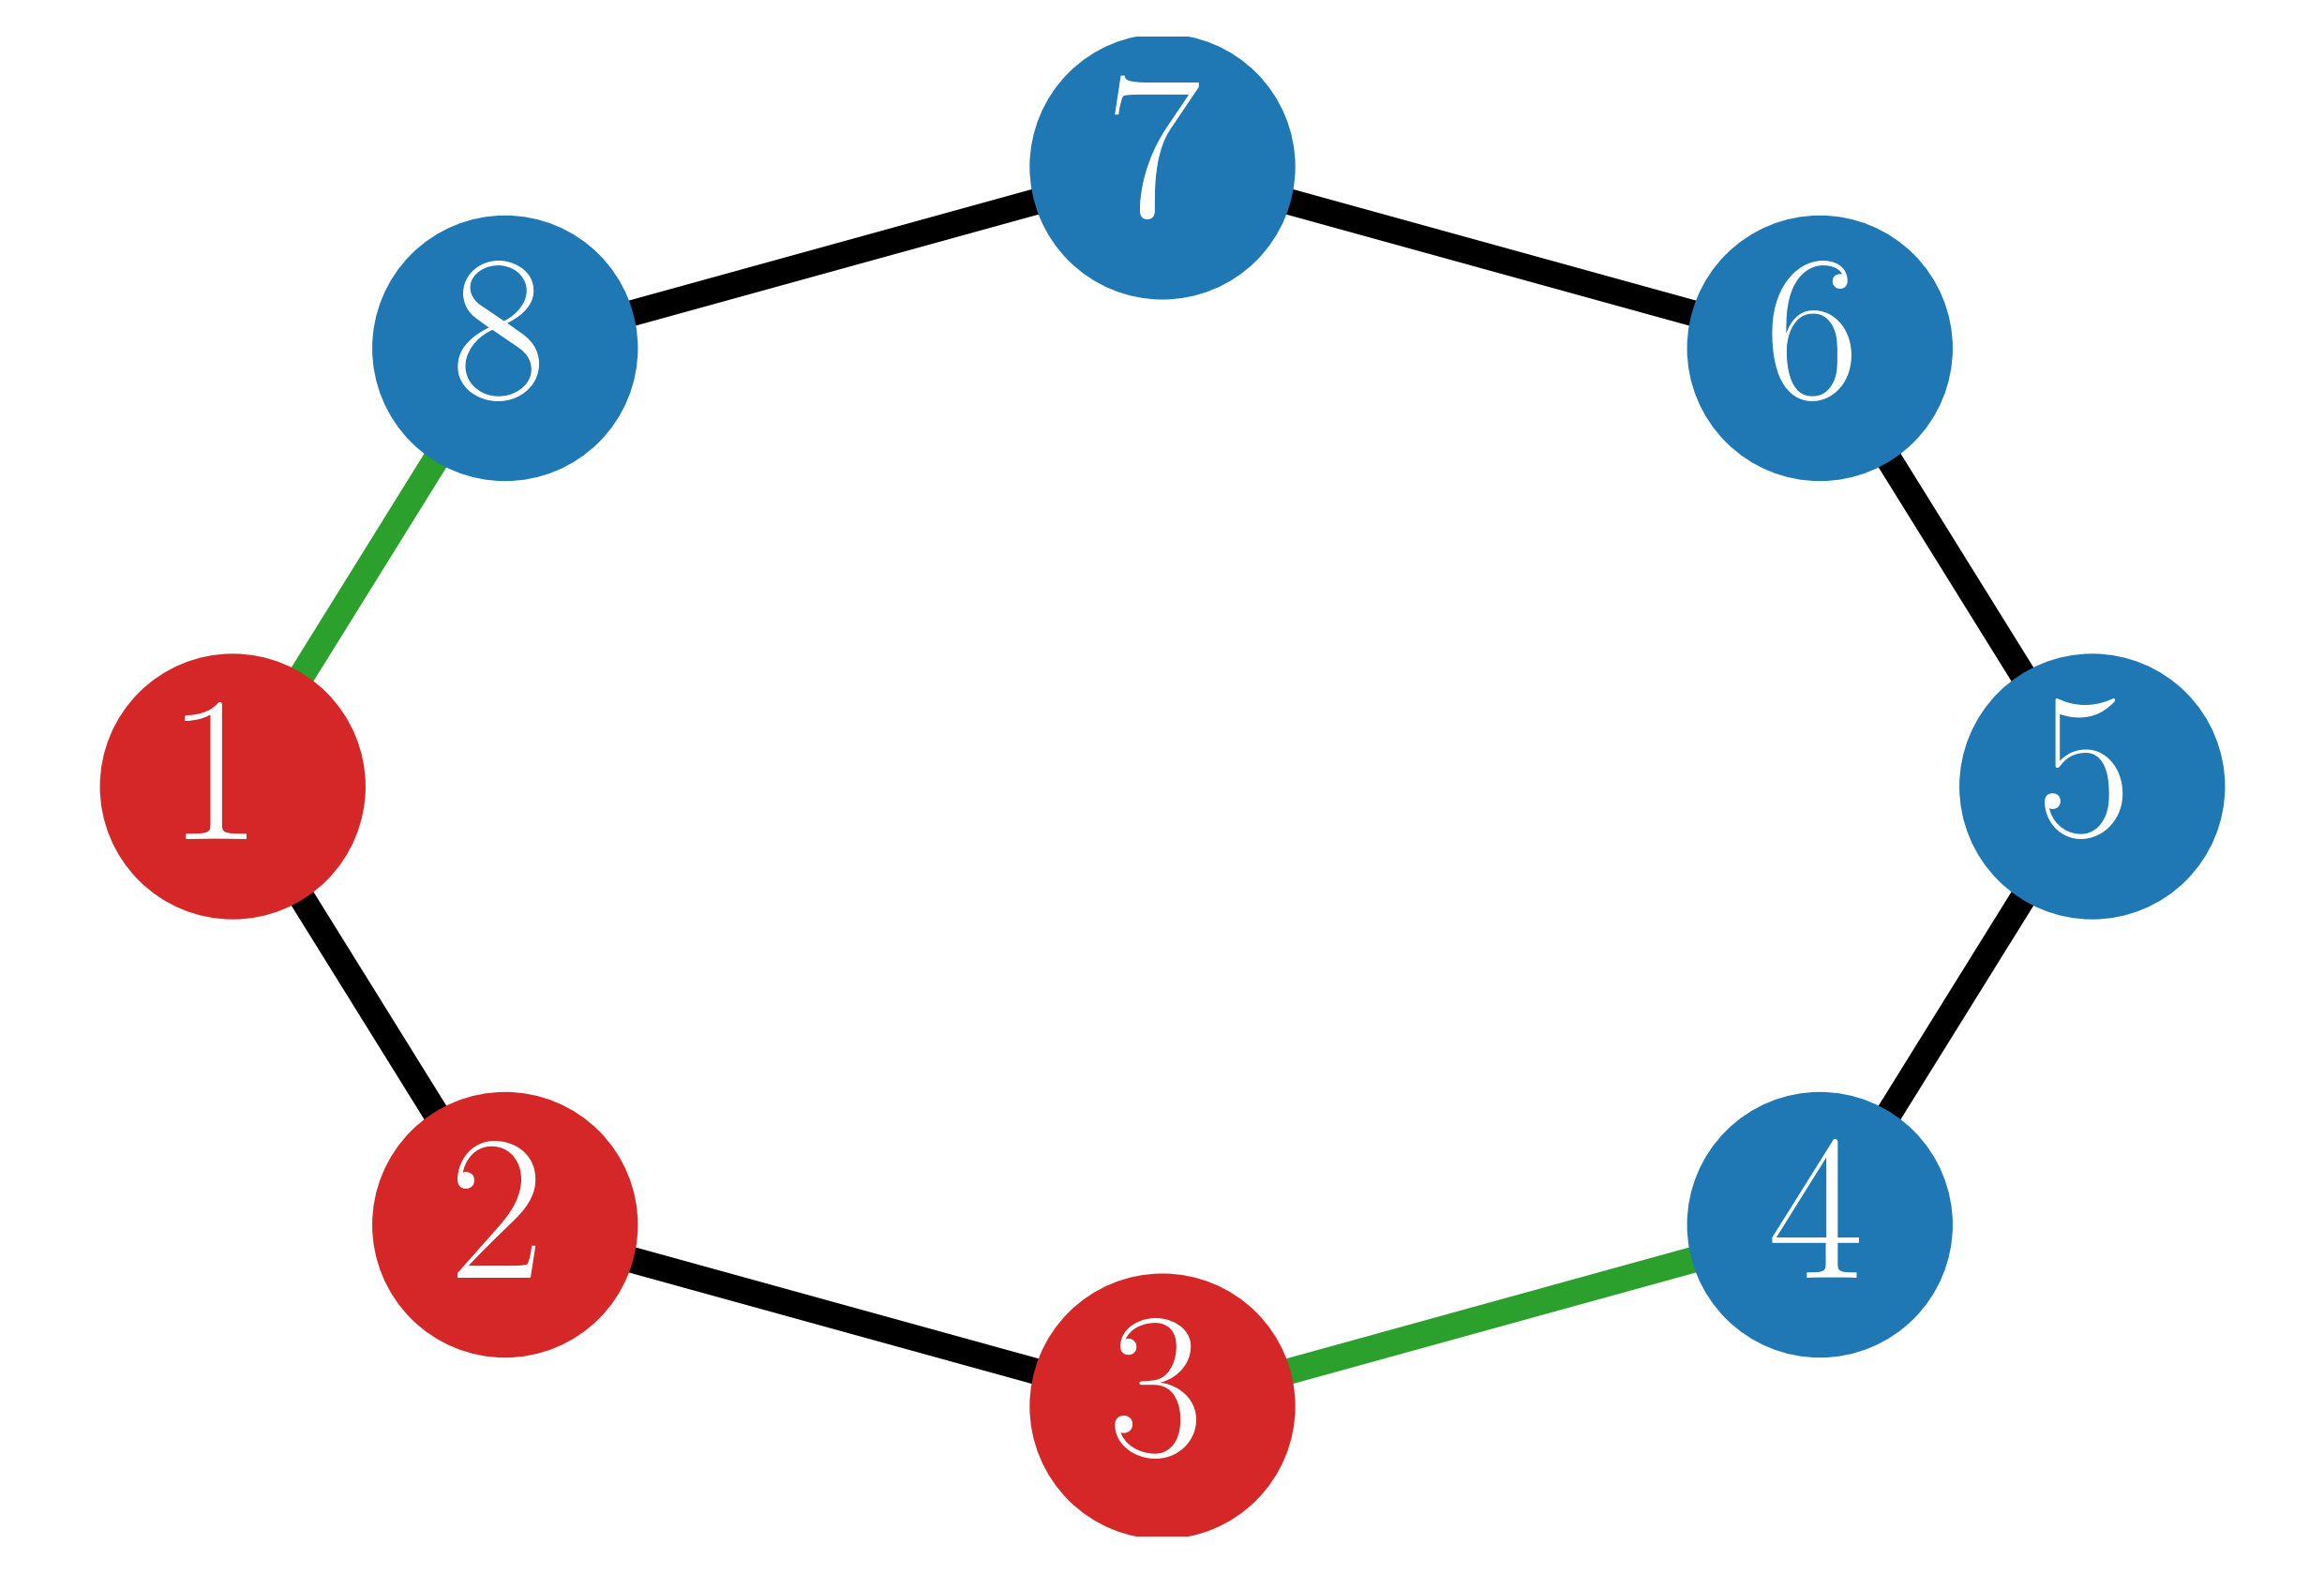
\includegraphics[width=\textwidth]{./figures/static_ring_example_spread.png}
		\caption*{$t=1 - \epsilon$, for all small $\epsilon > 0$}
	\end{subfigure}
	\begin{subfigure}[b]{0.49\textwidth}
		\centering
		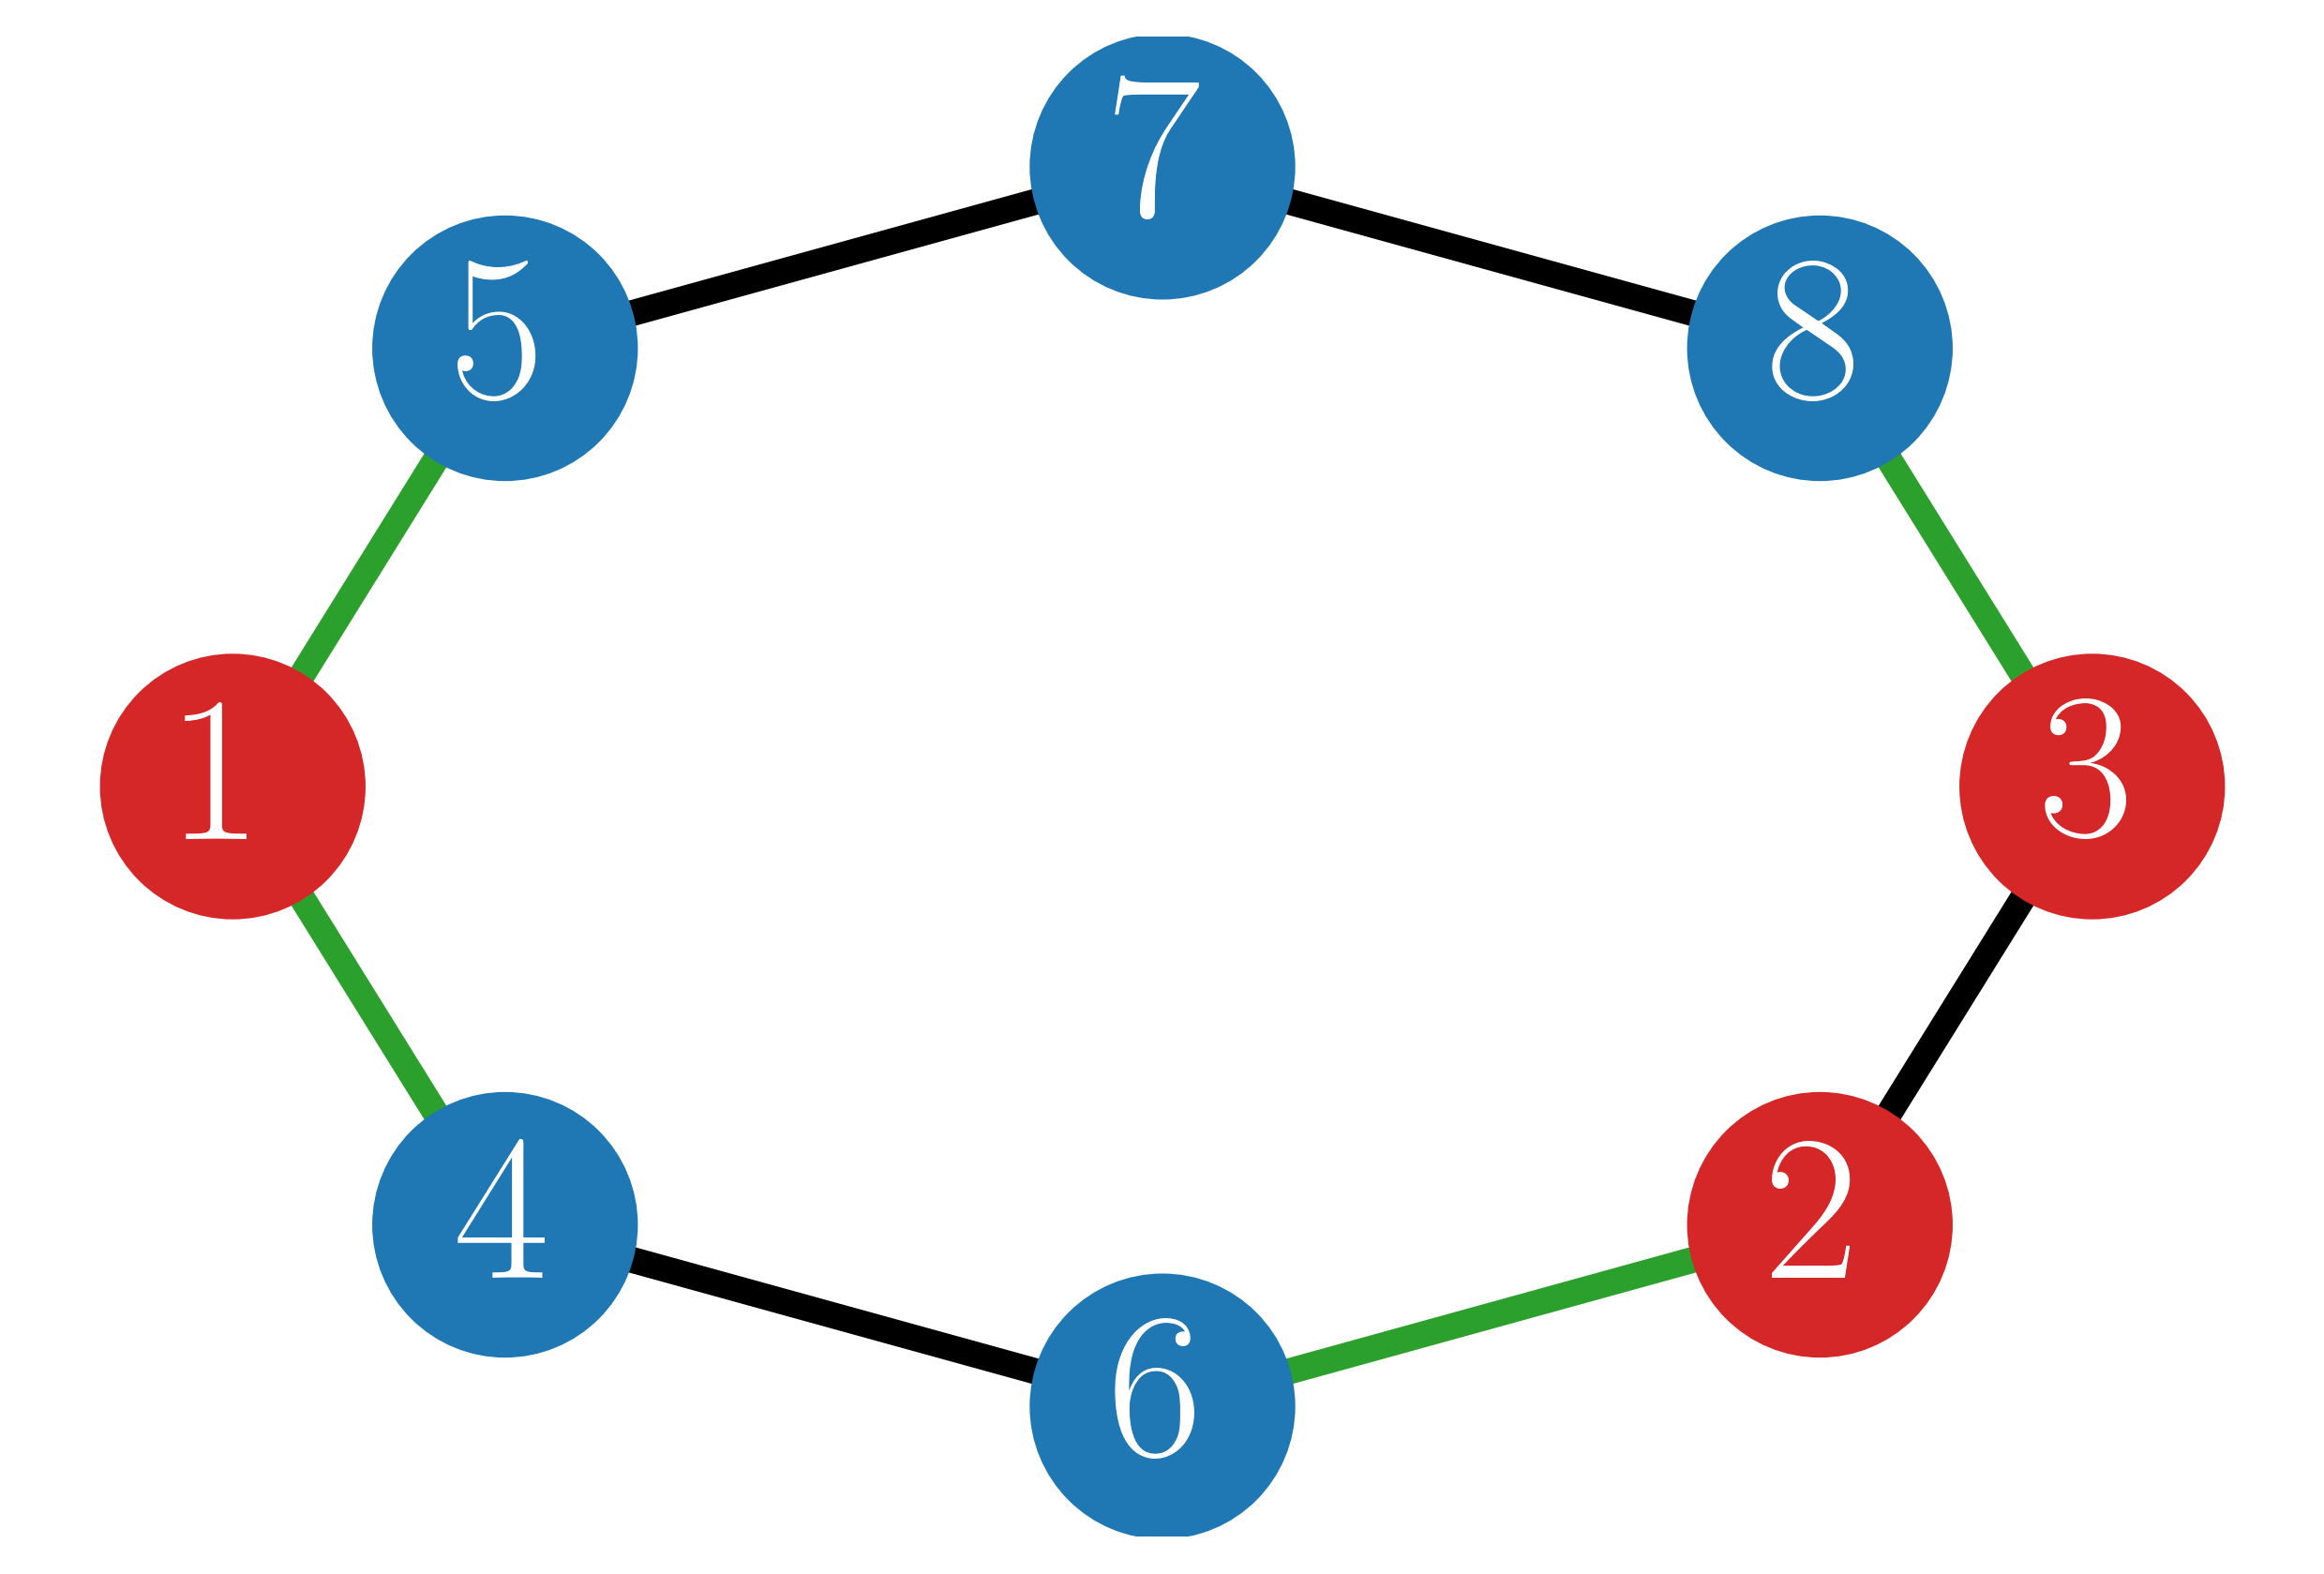
\includegraphics[width=\textwidth]{./figures/shuffled_ring_example_spread.png}
		\caption*{$t=1$}
	\end{subfigure}
	\caption{Example rumour spread on the Shuffled Ring Network}
	\label{fig:shuffledRingExampleSpread}
\end{figure}

Within a round, in the Shuffled Ring Network, the rumour spreads similarly to the Static Network, i.e. by extending the contiguous set of informed nodes. We see this behaviour in the $t = 1 - \epsilon$ case of Figure \ref{fig:shuffledRingExampleSpread}. However, when the network is shuffled at the start of the new round, it is likely that the continuous set of informed nodes is broken up and scattered around the ring, forming multiple continuous sets of informed nodes as seen in the $t=1$ case of Figure \ref{fig:shuffledRingExampleSpread}. Each of these new sets of adjacent informed nodes contributes an additional two active edges.

Hence, the spreading time is longer for the Static Ring Network, as the Static Ring Network is limited to 2 active edges at any time, whereas the Shuffled Ring Network could have many more.

\begin{figure}[h]
	\centering
	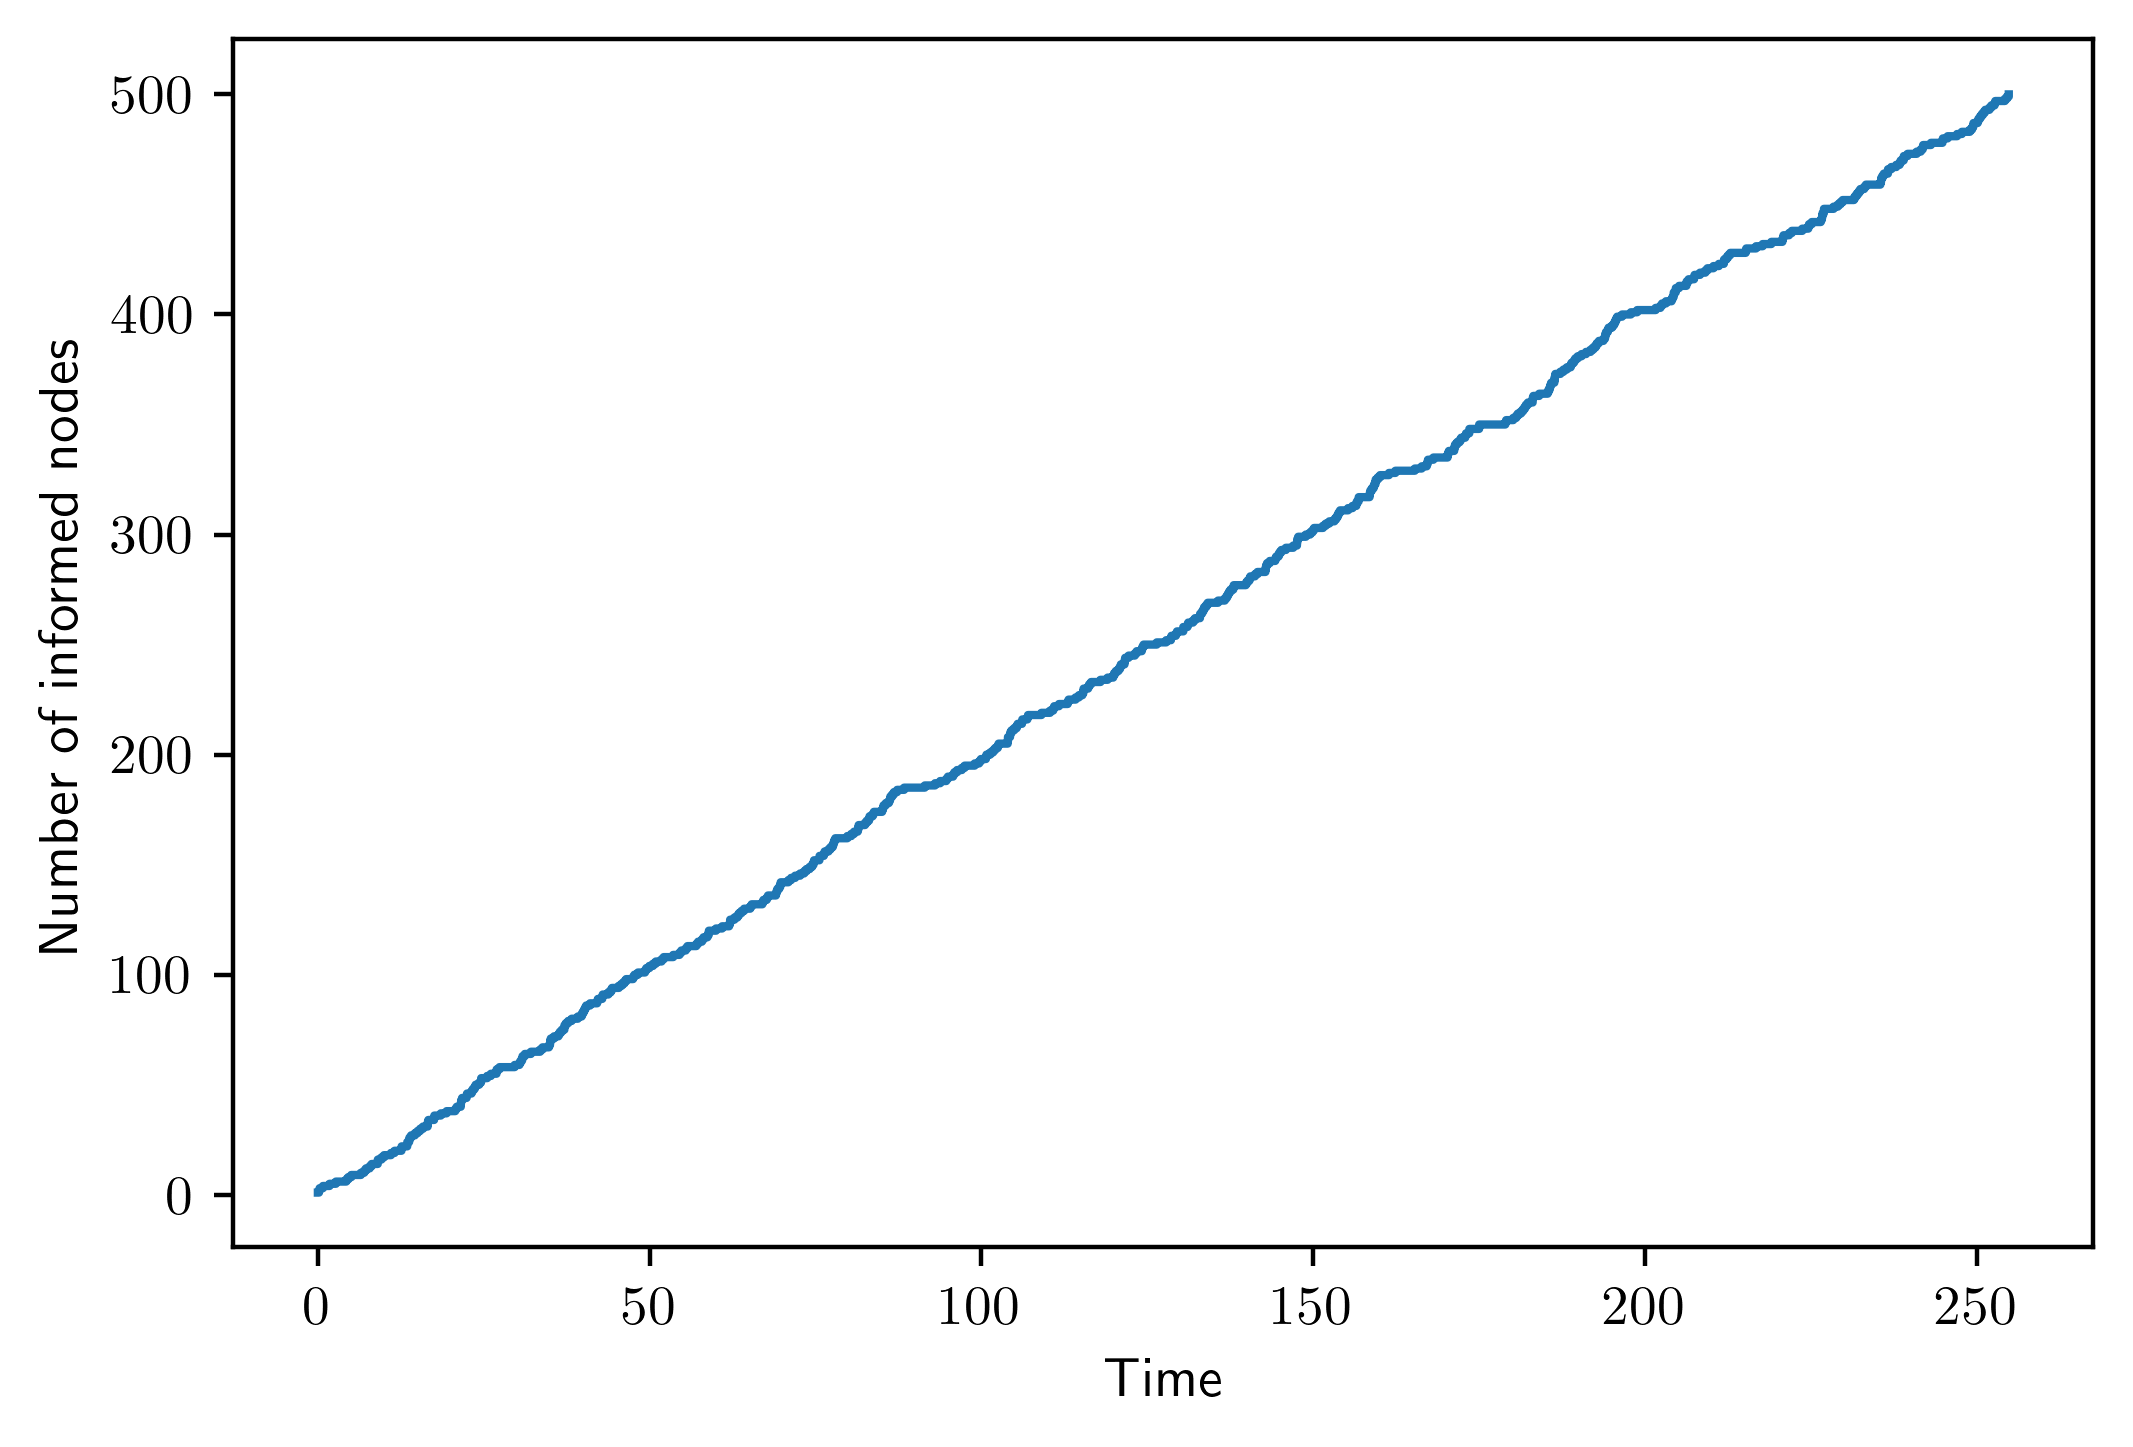
\includegraphics[width=\textwidth]{./figures/static_ring_informed_node_growth.png}
	\caption{Simulated informed node growth over time in the Static Ring Network}
	\label{fig:staticRingInformedNodeGrowth}
\end{figure}

We observe the described behaviour in the simulations. % TODO: Change this
Figure \ref{fig:staticRingInformedNodeGrowth} shows the number of informed nodes at each time during a rumour spread simulation on the Static Ring Network with 500 nodes. Notice that the rate at which the number of informed nodes increases is constant, since at all times there are exactly 2 active edges capable of spreading the rumour.

\begin{figure}[h]
	\centering
	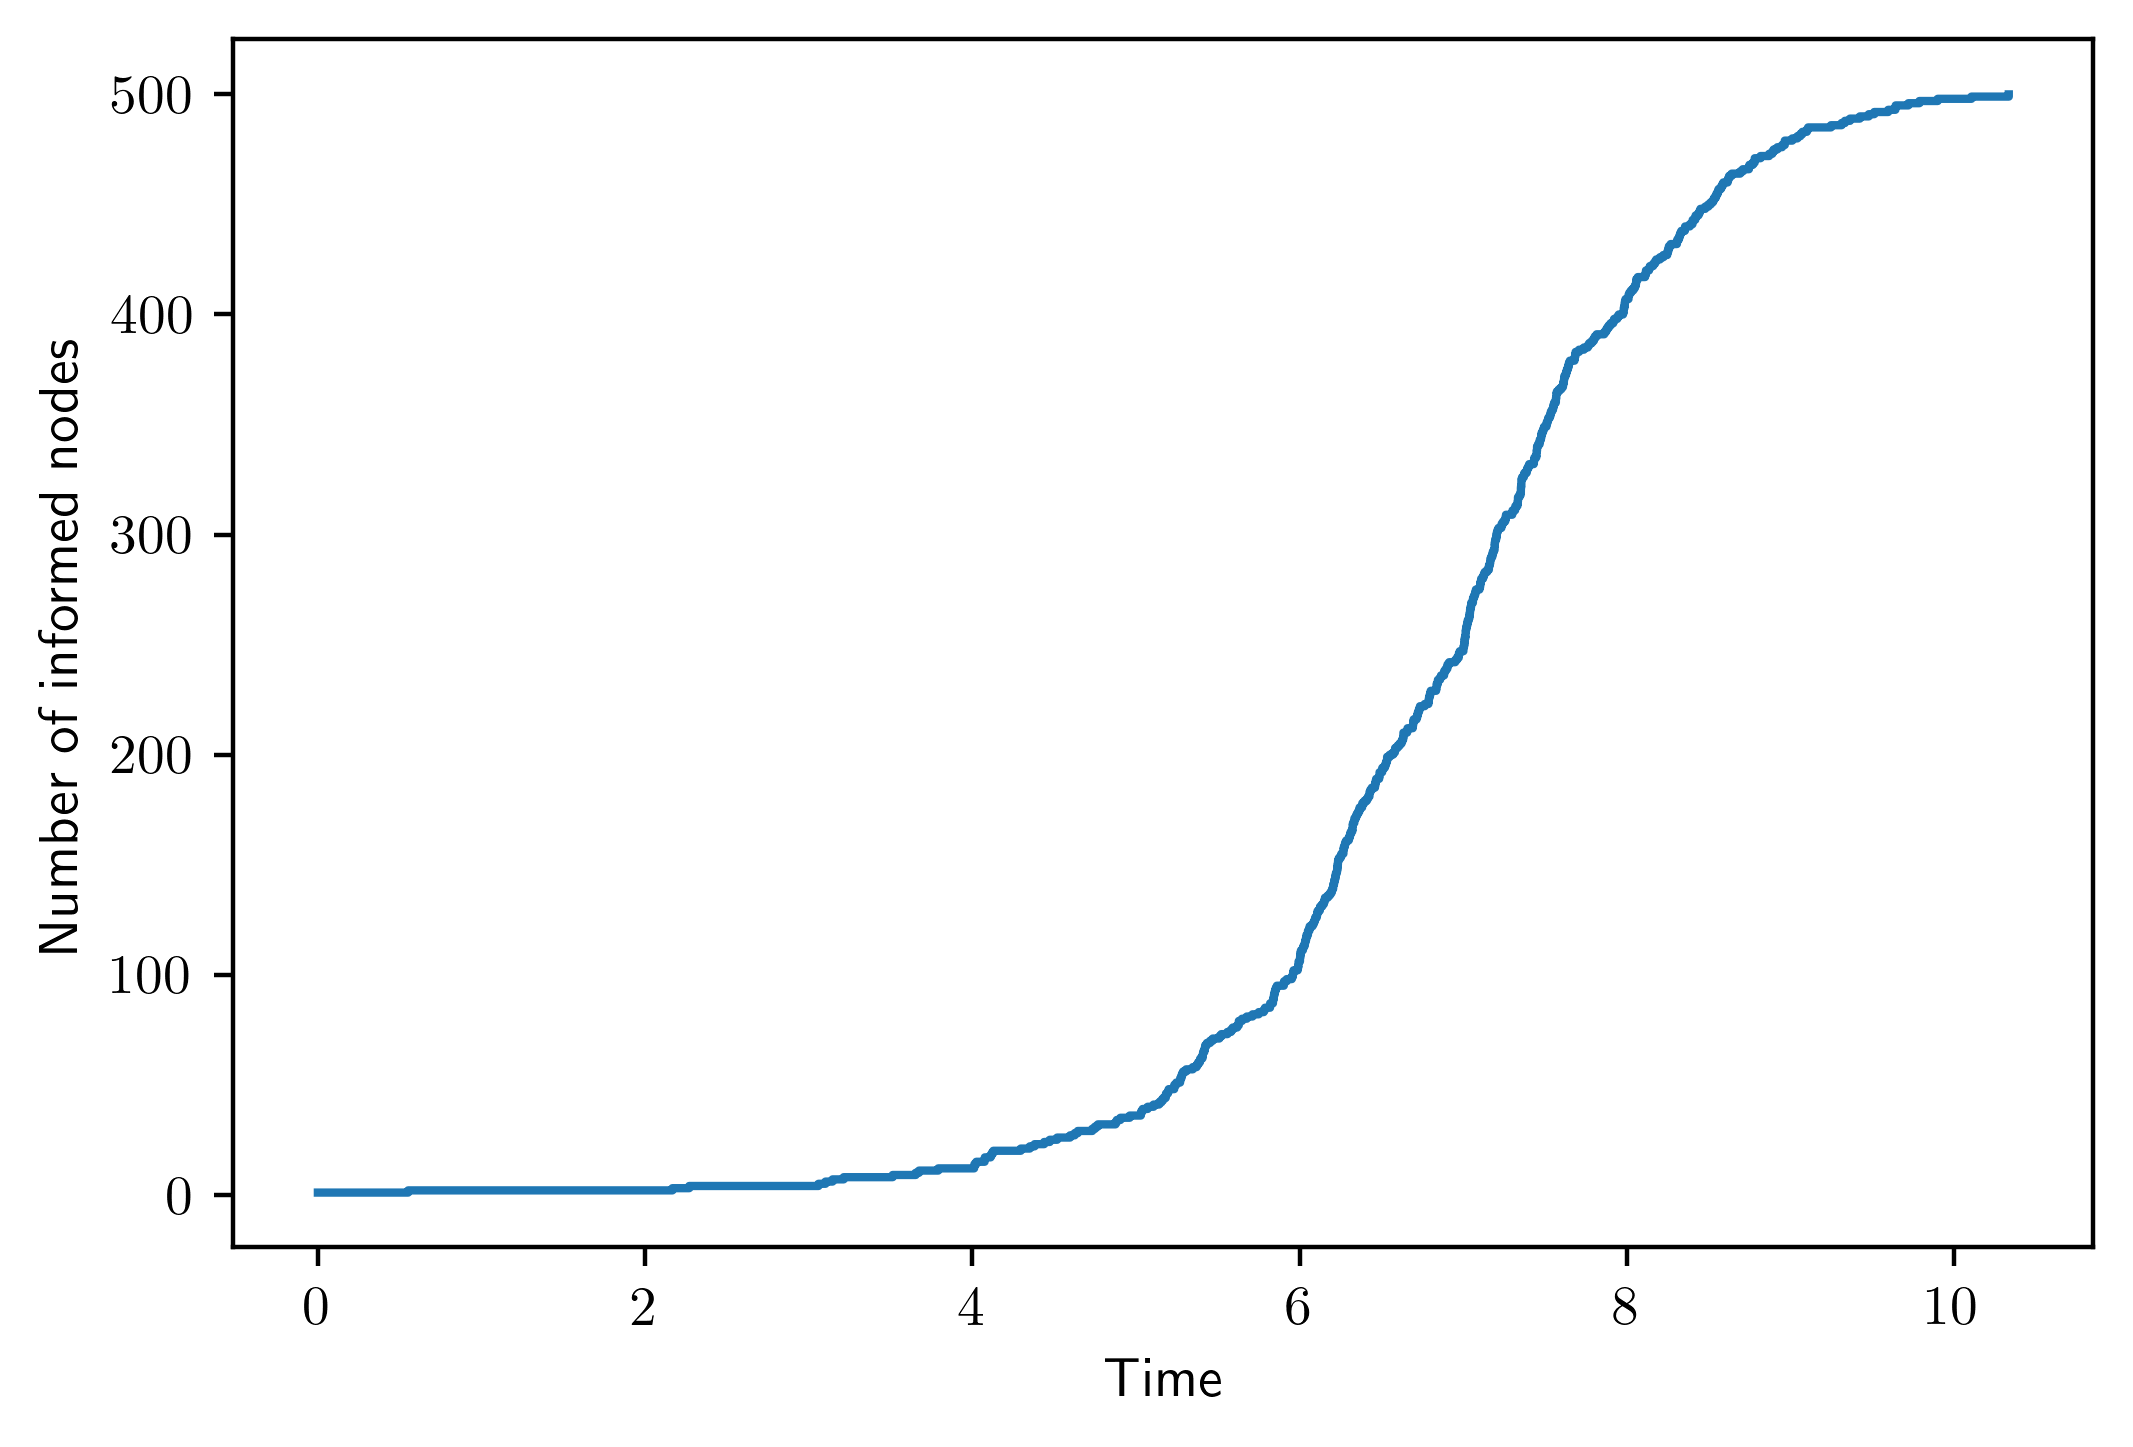
\includegraphics[width=\textwidth]{./figures/shuffled_ring_informed_node_growth.png}
	\caption{Simulated informed node growth over time in the Shuffled Ring Network}
	\label{fig:shuffledRingInformedNodeGrowth}
\end{figure}

Figure \ref{fig:shuffledRingInformedNodeGrowth} is a similar plot for a rumour spread on the Shuffled Ring Network. In this figure we note that the rate at which the number of informed nodes increases varies over time. In the first 3 rounds there are few informed nodes and only 3 opportunities for shuffling, hence the number of active edges is still close to 2. This is reflected in Figure \ref{fig:shuffledRingInformedNodeGrowth} by the initial slow growth in the number of informed nodes. However, after round 4 we see a rapid increase in the rate at which nodes are informed of the rumour, since there are a sufficient number of informed nodes for the shuffling to scatter informed nodes all around the ring, adding many active edges. 
As the network becomes saturated with informed nodes around time 7, the number of active edges begins to decrease as it becomes more likely that informed nodes will still be adjacent to other informed nodes after shuffling. Hence, in Figure \ref{fig:shuffledRingInformedNodeGrowth}, we see the rate of growth begins to decrease.

% TODO: Remove branching process - out of nowhere and unjustified?
This growth is similar to a branching process, where each set of contiguous informed nodes (the parent) has a probability of being split into multiple contiguous sets (the children). In this process the offspring distribution would change over time as the network becomes saturated. An interesting area for further study could be fully characterising this growth as a branching process.

Note that since Algorithm \ref{NodeCentricAsyncAlgorithm} is a random process, the individual simulations analysed in Figures \ref{fig:staticRingInformedNodeGrowth} and \ref{fig:shuffledRingInformedNodeGrowth} are not necessarily characteristic of how the rumour spreads on each network. However, after running the simulations multiple times, we see the same general structures we have discussed in both plots, hence these displays are useful illustrations.

We now return to the question posed in section \ref{subsect:shuffledRingAsyncApplication} - why is the bound given by Theorem \ref{theorem:AsyncUpperBound} weak for the Shuffled Ring? We saw in the proof of Theorem \ref{theorem:staticRingAsyncBound} that the $\mathcal{O}(n \log n)$ bound must hold w.h.p for both the Static Ring and Shuffled Ring, since they have identical structures. However, we have seen from simulations that the spreading time of the Static ring grows like $\mathcal{O}(n)$, so our bound for both the Static Ring and Shuffled Ring can be no better than $\mathcal{O}(n)$. 

We can interpret the Static Ring as a version of the Shuffled Ring in which the nodes have been relabelled. This example shows that such a renaming has no effect on the bound, but has a significant impact on the spreading time, hence the bound must accommodate for the network with the worse spreading time. We refer to such a network as "adversarial", in the sense that it is the network which aims to slow the spread of the rumour by relabelling nodes.

We refer to networks with the same topologies in each round up to the relabelling of nodes as "isomorphic". This example demonstrates a limitation of the bound: given a network, the bound can be no better than the spreading time of the corresponding adversarial network (the isomorphic network with the slowest spreading time).

For example, all other networks isomorphic but not equal to the Static Ring Network (such as the Shuffle Ring Network) involve some relabelling of nodes between rounds, which could introduce additional active edges. Thus, the Static Ring minimises the number of active edges at all time steps so is in fact the adversarial network for the Shuffle Ring Network. 

We saw in this example that the bound was only a factor of $\mathcal{O}(\log n)$ worse than the best possible bound in the adversarial case.  A natural question to ask is whether this is true in general: 
% TODO: Finish this

% TODO: introduce defns of active, inactive, ismorphism properly

% TODO: Example where the adversarial network doesn't impact - less symmmetry = more adverse effects??

% In adversarial cases bound is good - can it be better in general?
% TODO: Generalise

% TODO: Is the static always the adversarial? - No, about connectivity as well (shown in chapter 3)

% TODO: Adversarial not "figting back" but one of the possibilites the bound has to account for

% TODO: Difficult conductance requiring new techniques?